% !TeX root = ./main.tex

\documentclass[12pt]{report}
 
%%%%%%%%%%%%%%%%%%%%%%%%%%%%%%%%%%%%%%%%%%%%%%%%%%%%%%%%%%%%%%%%%%%%%%%%%%%%%%%%%%%%%%%
\usepackage[margin=1in]{geometry} 
\usepackage{amsmath,amsthm,amssymb}
\usepackage[utf8]{inputenc}
\usepackage{amsmath}
\usepackage[shortlabels]{enumitem}
\usepackage{mathtools}
\usepackage{amsfonts}
\usepackage{float}
\usepackage{chemmacros}
\usepackage{textalpha}
\usepackage[version=4]{mhchem}

\usepackage{epigraph}
\usepackage{lipsum}
\usepackage{parskip}
\usepackage[spanish,es-nodecimaldot]{babel}
\usepackage{tikz}
\usetikzlibrary{babel}
\usepackage{csquotes}
\usepackage{xcolor}
\usepackage[framemethod=tikz,xcolor=true]{mdframed}
\usepackage[new]{old-arrows}
%%%%%%%%%%%%%%%%%%%%%%%%%%%%%%%%%%%%%%%%%%%%%%%%%%%%%%%%%%%%%%%%%%%%%%%%%%%%%%%%%%%%%%%

%%%%%%%%%%%%%%%%%%%%%%%%%%%%%%%%%%%%%%%%%%%%%%%%%%%%%%%%%%%%%%%%%%%%%%%%%%%%%%%%%%%%%%%
% mis comandos
\usepackage{personalcommands}
\newtheorem{theorem}{Teorema}[chapter]
\newtheorem{lemma}[theorem]{Lema}
\newtheorem{prop}[theorem]{Proposición}
\newtheorem{coro}[theorem]{Corolario}
\newtheorem{conj}[theorem]{Conjetura}
\newtheorem{ejercicio}{Ejercicio}[section]
\newtheorem*{ejercicio*}{Ejercicio}
\theoremstyle{definition}
\newtheorem{definition}[theorem]{Definición}
\newtheorem{example}[theorem]{Ejemplo}
\theoremstyle{remark}
\newtheorem{remark}[theorem]{Nota}
\newtheorem{notacion}[theorem]{Notación}
\newcommand{\continuas}[1][]{\mathcal{C}^{ #1 }[a,b]}
\newcommand{\continuasabierto}[1][]{\mathcal{C}^{ #1 }(a,b)}
\newcommand{\soportecompacto}{\mathcal{D}(a,b)}
\newcommand{\xcero}{(a,b)}
\newcommand{\xcerocerrado}{[a,b]}
\newcommand{\fvariaciones}{F(x,y(x),y'(x))}
\newcommand*\circled[1]{\tikz[baseline=(char.base)]{\node[shape=circle,draw,inner sep=1pt] (char) {#1};}}
%%%%%%%%%%%%%%%%%%%%%%%%%%%%%%%%%%%%%%%%%%%%%%%%%%%%%%%%%%%%%%%%%%%%%%%%%%%%%%%%%%%%%%%
            
%%%%%%%%%%%%%%%%%%%%%%%%%%%%%%%%%%%%%%%%%%%%%%%%%%%%%%%%%%%%%%%%%%%%%%%%%%%%%%%%%%%%%%%
% Titulos
\makeatletter
\@ifundefined{@chapapp}{\def\@chapapp{\chaptername}}{}
\makeatother
\usepackage[Lenny]{fncychap}
\ChTitleVar{\Huge\bfseries}
\setcounter{chapter}{0}
%%%%%%%%%%%%%%%%%%%%%%%%%%%%%%%%%%%%%%%%%%%%%%%%%%%%%%%%%%%%%%%%%%%%%%%%%%%%%%%%%%%%%%%

%\renewcommand{\labelitemi}{{\tiny $\blacksquare$}}
\newcommand{\localtextbulletone}{\textcolor{black}{\raisebox{.45ex}{\rule{.6ex}{.6ex}}}}
\renewcommand{\labelitemi}{\localtextbulletone}
\begin{document}

\tableofcontents

%\chapter{Cálculo de variaciones}

\section{Herramientas previas y repaso}

Necesitaremos recordar algunas nociones y teoremas básicos sobre derivabilidad:

\begin{theorem}[derivada de una integral respecto de un parámetro]
\label{derivadaparametro}
Sea $X\subset\R^n$ y $(X,\mathcal{A},\mu)$ un espacio medible, $I$ un intervalo cerrado y sea $\funcion{f}{I\times X}{\R}$ tal que:

\begin{enumerate}[(a)]
\item $\forall t \in I$, $x\mapsto f(t,x)$ es integrable.
\item $\forall x\in X$, la función $t\mapsto f(t,x)$ es derivable en $t\in I$.
\item Existe $\funcion{g}{X}{\R}$ integrable tal que
\[
\left|\derivada{f}{t}(t,x)\right|\leq |g(x)| \espacio \forall x\in X\; \forall t \in I
\]
Entonces la función $F(t)=\int_Xf(t,x)dx$ es derivable en $t_0$ y la derivada es 
\[
F'(t_0)=\displaystyle\int_X\derivada{f}{t}(t_0,x)dx
\]
\end{enumerate}

\end{theorem}

TODO: añadir resto de resultados usados de otras asignaturas que no recordábamos

\section{Problema general del cálculo de variaciones}

Primeramente definimos un tipo de funciones llamadas \textit{funciones test} o \textit{funciones de la clase de Schwartz}, junto con algunos resultados que usaremos bastante para trabajar con ellas.

\begin{definition}
\label{funcionestest}
Dado $I$ intervalo, se llama \textit{espacio de funciones test} al conjunto:
\[
\mathcal{D} = \mathcal{D}(a,b) = \{\phi\in C^{\infty}(a,b): \; \exists J\subset(a,b) \text{ compacto: } \phi(x)=0 \text{ si } x \notin J\}
\]
\end{definition}

\begin{lemma}
\label{existenciaphi}
Dado $x_0\in(a,b)$ y $\varepsilon>0$ tal que $[x_0-\varepsilon, x_0+\varepsilon]\subset(a,b)$, existe $\phi\in\mathcal{D}(a,b)$ tal que $\phi(x)>0$ si $x\in(x_0-\varepsilon,x_0+\varepsilon)$ y $\phi(x)=0$ en otro caso.
\end{lemma}

\begin{proof}
La demostración la vamos a hacer por construcción. Sea $\funcion{g}{\R}{\R}$ definida por:
\[
g(x)=\left\{
\begin{array}{cc}
e^{1/x} & x<0 \\
0 & x\geq 0
\end{array}
\right.
\]
Tenemos que $\limite{x}{0^-}{g(x)}=0$, luego $g$ es continua. Veamos que de hecho $g\in C^{\infty}$. Su derivada es:
\[
g'(x)=\left\{
\begin{array}{cc}
e^{1/x}\left(-\frac{1}{x^2}\right) & x<0 \\
0 & x> 0
\end{array}
\right.
\]
Mediante un proceso iterativo llegamos a:
\[
g^{n)}(x)=\left\{
\begin{array}{cc}
e^{1/x}\frac{R(x)}{x^{2n}} & x<0 \\
0 & x> 0
\end{array}
\right.
\]
donde $R(x)$ es un cierto polinomio que no nos interesa calcular. Queremos ver que 
\[\limite{x}{0^-}{g^{n)}(x)}=0,\]
con lo cual, $g\in C^n$. Haciendo el cambio $y=-\frac{1}{x}$, el anterior límite equivale a 
\[
\limite{y}{+\infty}{\frac{y^{2n}}{e^y}}=0 \Rightarrow g\in C^{n} \;\forall n \in\N \Rightarrow g\in C^{\infty}
\]
Con lo anterior, solo nos queda definir la función buscada de forma que sea una función test, es decir, la definimos como:
\[
\phi(x)=g(x-(x_0+\varepsilon))g((x_0-\varepsilon)-x) \espacio \varepsilon>0 
\]

\end{proof}


\begin{theorem}
\label{theorem:1.3}
Sea $f\in \continuas$ tal que
\[
\int f(x)\phi(x)dx=0 \hspace{1cm} \forall \phi \in \soportecompacto
\]
Entonces $f(x)=0 \;$  $\forall x\in [a,b]$.
\end{theorem}

\begin{proof}
Sea $\bar{x}\in \xcero$ y supongamos por reducción al absurdo que $f(\bar{x})\neq 0$. Podemos suponer $f(\bar{x})>0$. Aplicando el teorema de conservación del signo, obtenemos $\varepsilon>0$ tal que $f(x)>0 \text{ si } x \in (\bar{x}-\varepsilon,\bar{x}+\varepsilon)$.

Por el lema \ref{existenciaphi}, existe una función test $\phi$ tal que $\phi(x)>0$ si $x\in(\bar{x}-\varepsilon, \bar{x}+\varepsilon)$ y $0$ en otro caso. Luego:
\[
0=\int_{a}^{b}f(x)\phi(x)dx=\int_{\bar{x}-\varepsilon}^{\bar{x}+\varepsilon}f(x)\phi(x)dx>0 \Rightarrow f(\bar{x})=0
\]
Como $\bar{x}$ era arbitrario, tenemos que $f(\bar{x})=0 \; \forall \bar{x}\in\xcero$, y por la continuidad de $f$ podemos extenderlo a los extremos también, es decir, $f(a)=f(b)=0$.

\end{proof}

\subsection{Cálculo de extremales}

Sea $\Omega\subset\R^3$, definamos $F:\Omega \longrightarrow \R$ tal que $(x,y,p)\longmapsto F(x,y,p)$. Supongamos que $F\in C^1(\Omega)$  respecto de las dos últimas variables, es decir, existen $\derivada{F}{y}$ y $\derivada{F}{p}$, continuas. 

Usando la función anterior, podemos definir el siguiente funcional:

\begin{equation}\label{funcional}
L(y) = \int_{a}^{b}\fvariaciones dx 
\end{equation}


Nuestro objetivo en este apartado será encontrar \textit{extremales} de ese funcional, es decir, máximos o mínimos.

\begin{notacion}
Normalmente, a las derivadas parciales las denotaremos por:
\[
\derivada{F}{x}=F_x
\]
\end{notacion}

Los \textit{extremales} los buscaremos entre los elementos de un conjunto de funciones cumpliendo ciertas propiedades:

\begin{definition}
\label{espaciofuncionesbuenas}

Sea $\Omega\subset\R^3$ y $F:\Omega\longrightarrow \R$ funcional en las condiciones anteriores. Definimos entonces el siguiente conjunto:

\begin{equation}\label{espaciofunciones}
D=\{y\in\continuasabierto\cap\continuas[1]: \text{ se cumplen (a),(b) y (c)}\}
\end{equation}

\begin{enumerate}[(a)]
\item $(x,y(x),y'(x))\in\Omega \espacio \forall x\in\xcero$
\item $y(a)=y_0$ e $y(b)=y_1$ (\textit{Condición de contorno})
\item $\displaystyle\int_{a}^b\Big|\fvariaciones\Big|dx<+\infty$ 
\end{enumerate}

\end{definition}

El siguiente teorema nos proporcionará una condición sobre las derivadas parciales de $F$, que nos ayudará a buscar \textit{extremales}. Para su demostración necesitaremos el siguiente lema:

\begin{lemma}
\label{lemmatecnico}
Sea $\{s_n\}\longrightarrow 0$ una sucesión de números reales y $\phi\in \soportecompacto$, existe $n_0\in\N$ tal que si $y\in D$, entonces $y+s_n\phi\in D \espacio \forall n\geq n_0$.
\end{lemma}
\begin{proof}

Sea $\phi\in\soportecompacto$ y $K=\supp\phi$.Tenemos que comprobar que $y+s_n\phi$ cumple las condiciones de la definición \ref{espaciofuncionesbuenas}.

\begin{enumerate}[(a)]
\item Razonemos por reducción al absurdo. Supongamos que hay infinitos valores de $n\in\mathbb{N}$ tales que $(x_n,y(x_n)+s_n\phi(x_n),y'(x_n)+s_n\phi'(x_n))\notin \Omega$ para algún $x_n\in(a,b)$. Tomando una parcial si es necesario, podemos suponer una sucesión $\{x_n\}$ tal que para cada $n\in\mathbb{N}$, $(x_n,y(x_n)+s_n\phi(x_n),y'(x_n)+s_n\phi'(x_n))\notin \Omega \Rightarrow x_n\in\supp\phi$, ya que si no estuviera, tendríamos que $\phi(x_n)=0$ y $(x_n,y(x_n),y'(x_n))\in \Omega$. Como el soporte es compacto, podemos suponer que $\{x_n\}\longrightarrow\bar{x}\in\supp\phi\in(a,b)$. Si tomamos límite:
\[
\limitemasinfinito{n}{(x_n,y(x_n)+s_n\phi(x_n),y'(x_n)+s_n\phi'(x_n))}=(\bar{x},y(\bar{x}),y'(\bar{x}))\notin\Omega 
\]
porque el complementario de $\Omega$ es cerrado y el límite se queda fuera, llegando así a un absurdo. Por tanto, debe existir un $n_0\in\mathbb{N}$ tal que $(x_n,y(x_n)+s_n\phi(x_n),y'(x_n)+s_n\phi'(x_n))\in \Omega\quad\forall n\geq n_0$.
\item Evidente, ya que $\phi(a)=\phi(b)=0$.
\item Tomando $n\geq n_0$,de (a) tenemos:
\[
\integral{a}{b}{\Big|F(x,y(x)+s_n\phi(x),y'(x)+s_n\phi'(x))\Big|dx}=\]
\[
=\integral{(a,b)\backslash K}{}{\Big|F(...)\Big|dx}+\integral{K}{}{\Big|F(...)\Big|dx} < +\infty
\]
El primer término es finito ya que, fuera de $K$, $\phi=0$, luego ese término coincide con $\integral{(a,b)\backslash K}{}{\Big|F(x,y(x),y'(x))\Big|dx}$, que
es finito porque $y\in D$.
El segundo término lo es porque ser la integal de una función continua en un compacto. 
\end{enumerate}
\end{proof}
Lo que nos asegura este lema es que podamos sumar una perturbación \textit{pequeña} a nuestro extremal sin \textit{salirnos} de $D$.

\begin{theorem}
\label{theorem:1.7}
Si $\bar{y}\in D$ es un extremal, entonces:
\[
\integral{a}{b}{F_y(x,\bar{y}(x), \bar{y}'(x))}\phi(x)dx+\integral{a}{b}{F_p(x,\bar{y}(x), \bar{y}'(x))}\phi'(x)dx=0 \espacio \forall \phi\in \soportecompacto
\]
A $\bar{y}$ se le suele llamar \textbf{función crítica}.
\end{theorem}

\begin{proof}
Sean $\bar{y}\in D$ extremal y $\phi\in\soportecompacto$. Definimos el funcional $g:\R\longrightarrow\R$ tal que $g(s)=L(\bar{y}+s\phi)$.

Por el lema anterior, existe $\varepsilon>0$ tal que $g$ está bien definida en $(-\varepsilon,\varepsilon)$.

Ahora queremos derivar $g$ respecto de $s$, pero necesitamos que esté definida en un intervalo cerrado (por el teorema \ref{derivadaparametro}). Para ello, tomamos un intervalo cerrado $J$ de forma que $\supp (\phi)\subset J\subset [a,b]$. 

Derivamos $g$ respecto de $s$:
\[
g'(s)=\left(
\integral{[a,b]}{}{F(x,\bar{y}+s\phi(x),\bar{y}'+s\phi'(x))dx}
\right)'=
\]
\[
=\left(
\integral{[a,b]\backslash J}{}{F(x,\bar{y}+s\phi(x),\bar{y}'+s\phi'(x))dx}+
\integral{J}{}{F(x,\bar{y}+s\phi(x),\bar{y}'+s\phi'(x))dx}
\right)'
\]
Usando que $\integral{[a,b]\backslash J}{}{F(x,\bar{y}+s\phi(x),\bar{y}'+s\phi'(x))dx}\phi(x)$ es una constante (por que $\bar{y}\in D$ y $\phi = 0$ en $[a,b]\backslash J$) cuya derivada es cero, obtenemos que:
\[
g'(s)= \integral{J}{}{\Big(F_y(x,\bar{y}+s\phi(x),\bar{y}'+s\phi'(x))\phi(x)+F_p(x,\bar{y}+s\phi(x),\bar{y}'+s\phi'(x))\phi'(x)\Big)dx}
\]
Como $\phi=0=\phi'$ fuera de $J$
\[
g'(s)= \integral{[a,b]}{}{\Big(F_y(x,\bar{y}+s\phi(x),\bar{y}'+s\phi'(x))\phi(x)+F_p(x,\bar{y}+s\phi(x),\bar{y}'+s\phi'(x))\phi'(x)\Big)dx}
\]
Si evaluamos ahora $g'$ en 0 y usamos que $\bar{y}$ es extremal, tenemos:
\[
g'(0)=\integral{a}{b}{\Big(F_y(x,\bar{y},\bar{y}')\phi+F_p(x,\bar{y},\bar{y}')\phi'\Big)dx}=0 
\]
\end{proof}

\subsection{Ecuación de Euler}

Usando el teorema anterior vamos a llegar a una ecuación diferencial de segundo orden que nos ayudará a resolver este problema. Definimos $Z(x)=F_p(x,y(x),y'(x))$, nuestro objetivo ahora es imponer condiciones suficientes para que $Z(x)\in C^1(a,b)$, para poder derivarla y obtener una ecuación diferencial en $y'$.

Para continuar necesitamos un lema previo:

\begin{lemma}
Sea $Z\in C^1(x_0,x_1)$, entonces:
\[
\integral{a}{b}{Z(x)\phi'(x)dx}=-\integral{a}{b}{Z'(x)\phi(x)dx} \espacio \forall \phi\in\soportecompacto
\]
\end{lemma}

\begin{proof}

Resolviendo la integal por partes tenemos:
\[
\left.\begin{array}{cc}
u=Z(x) & du=Z'(x)dx\\
dv=\phi'(x)dx & v=\phi
\end{array}\right\} \Rightarrow\integral{a}{b}{Z(x)\phi'(x)dx}=Z(x)\phi(x)\Big|_a^b-\integral{a}{b}{Z'(x)\phi(x)dx}=
\]
\[
=-\integral{a}{b}{Z'(x)\phi(x)dx}
\]

\end{proof}

Este lema nos permite \enquote{intercambiar la derivada de sitio}.
Usando ahora el Teorema \ref{theorem:1.7} (podemos usarlo porque $y$ es función crítica) y el lema anterior, tenemos:
\[
0=\integral{a}{b}{F_y(x,y, y')}\phi(x)dx+\integral{a}{b}{F_p(x,y,y')}\phi'(x)dx= 
\]
\[
=\integral{a}{b}{F_y(x,y, y')}\phi(x)dx+\integral{a}{b}{Z(x)}\phi'(x)dx=
\]
\[
=\integral{a}{b}{F_y(x,y, y')}\phi(x)dx-\integral{a}{b}{Z'(x)}\phi(x)dx=
\]
\[
=\integral{a}{b}{\Big(F_y(x,y, y')-Z'(x)\Big)}\phi(x)dx=0 \espacio \forall\phi\in\soportecompacto
\]
Y usando ahora el Teorema \ref{theorem:1.3} nos queda:
\[
F_y(x,y,y')-Z'(x)=0 \espacio \forall x \in\xcero
\]
Que denoteramos por:
\[
\frac{d}{dx}F_p-F_y(x,y,y')=0 \espacio \textbf{(Ecuación de Euler)}
\]
Las condiciones sobre $F$ se pueden rebajar con el siguiente teorema:

\begin{theorem} 
\label{theorem:12}
Si $F\in C^1_{yp}$, $y'\in C^1$, función crítica, entonces:
\[
Z(x)=F_p(x,y(x),y'(x))\in C^1
\]
\[
Z'(x)=F_y(x,y(x),y'(x))
\]
\end{theorem}

Ya tenemos la ecuación que queremos resolver. La demostración del teorema es consecuencia de los anteriores resultados.

\begin{definition}
Una función $\phi\in\soportecompacto$ admite primitiva si existe otra función $\Psi\in\soportecompacto$ tal que $\Psi'=\phi$. 
\end{definition}

\begin{lemma}
\label{lemma:13}
Sea $\phi\in\mathcal{D}(a,b)$, entonces:
\[
\phi \text{ admite primitiva } \Longleftrightarrow \integral{a}{b}{\phi(x)dx}=0
\]
\end{lemma}

\begin{proof}
\hfill\\
$(\Rightarrow)$ Por hipótesis, supongamos que existe $\Psi$ tal que $\phi=\Psi'$. Ahora solo tenemos que integrarla y usar que $\Psi$ vale 0 en los extremos por ser una función de soporte compacto:
\[
\integral{a}{b}{\phi(s)ds}=\integral{a}{b}{\Psi'(s)ds}=\Psi\Big|_a^b=0
\]
$(\Leftarrow)$  Si $\integral{a}{b}{\phi(s)ds}=0$, entonces tenemos la siguiente situación: $\supp\phi\subset[a',b']$ tal que $a<a'\leq b'<b$.

\begin{center}
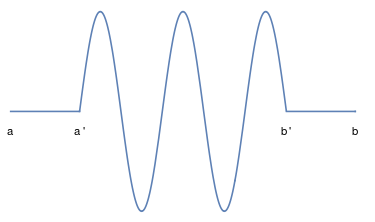
\includegraphics[scale=0.4]{./img/testfuncion.png}
\end{center}

Definimos $\Psi(x)=\integral{a'}{x}{\phi(s)ds}$ y tenemos $\Psi'=\phi$. Falta probar que $\Psi\in\mathcal{D}(a,b)$.
Si $x\leq a'$, claramente $\Psi(x)=0$ \big($\phi(x)=0\quad\forall x\in(a,a')$\big). Si $x\geq b'$,
\[
\int_{a'}^x\phi(s)ds=\int_{a'}^{b'}\phi(s)ds=\int_{a}^{b}\phi(s)ds=0
\]
Por tanto $\supp\Psi\subset[a',b']$.

\end{proof}

\begin{lemma}
\label{lemma:14}
Sea $f\in C(a,b)$ tal que $\integral{a}{b}{f(x)\phi'(x)dx=0}\espacio\forall\phi\in\mathcal{D}(a,b)\Longrightarrow f \text{ es constante.}$
\end{lemma}

\begin{proof}
Sea $x_0\in(a,b)$, tomamos una función $\phi_{x_0}\in \soportecompacto$ cumpliendo la tesis del lema \ref{existenciaphi}. Podemos tomarla de forma que $\integral{a}{b}{\phi_{x_0}(s)ds}=1$ (multiplicándola por cierta constante). 

Definimos $\Psi(x)=\integral{a}{x}{\phi_{x_0}(s)ds}$ y tomamos $c$ de forma que:
\[
\integral{a}{b}{f(s)\Psi'(s)}=c\integral{a}{b}{\Psi'(s)ds}=c\Psi\Big|_a^b=c
\]
Tomamos $\phi\in\soportecompacto$ y veamos que la función $\phi-\lambda\Psi'$ tiene primitiva para cierto $\lambda\in\R$. Supongamos que tiene media 0, y despejemos $\lambda$:
\[
\integral{a}{b}{\phi(s)-\lambda\Psi'(s)}=0 \Longrightarrow \lambda=\integral{a}{b}{\phi(s)ds}
\]
Haciéndo esa elección de $\lambda$, $\phi-\lambda\Psi'$ tiene primitiva por el lema \ref{lemma:13}.
\[
0=\integral{a}{b}{f(s)(\phi(s)-\lambda\Psi'(s))ds}=\integral{a}{b}{f(s)\phi(s)ds}-\lambda\integral{a}{b}{f(s)\Psi'(s)ds}=
\]
\[
=\integral{a}{b}{f(s)\phi(s)ds}-c\integral{a}{b}{\phi(s)ds}=\integral{a}{b}{(f(s)-c)\phi(s)ds} \Rightarrow f(s)-c=0 \Rightarrow f\equiv c
\]
\end{proof}

\begin{lemma}
Sean $f$,$g$ funciones continuas en $(a,b)$, entonces es equivalente:
\[
\integral{a}{b}{g\phi}+\integral{a}{b}{f\phi'}=0 \espacio \forall\phi\in\soportecompacto \Longleftrightarrow f\in C^1(a,b), g=f'
\]
\end{lemma}

\begin{proof}

($\Rightarrow$)Tomamos $x_0\in(a,b)$ y definimos $\tilde{f}(x)=\integral{a}{x}{g(s)ds}\Rightarrow \tilde{f}\in C^1$.
\[
\integral{a}{b}{\tilde{f}(s)\phi'(s)+g(s)\phi(s)ds}=\integral{a}{b}{\tilde{f}(s)\phi'(s)+\tilde{f}'(s)\phi(s)ds}=\integral{a}{b}{(\tilde{f}\phi)}=\tilde{f}\phi\Big|_a^b=0
\]
Restando la expresión de la hipótesis menos la anterior, obtenemos:
\[
0=\integral{a}{b}{f(s)\phi'(s)ds}-\integral{a}{b}{\tilde{f}(s)\phi'(s)ds}=\integral{a}{b}{(f-\tilde{f})(s)\phi'(s)ds}
\]
Y usnado el lema \ref{lemma:14}, tenemos que $f-\tilde{f}$ es constante, luego $f\in C^1$ ya que $\tilde{f}$ también pertenece a $C^1$.

($\Leftarrow$) 
\[
0=f\phi(x)\Big|_a^b=\integral{a}{b}{(f(x)\phi(x))'dx}=\integral{a}{b}{f(x)\phi'(x)dx+f'(x)\phi(x)dx}
\]
\end{proof}

\section{Problema de Braquistocrona}

Este problema se centra principalmente en averiguar que forma (curva) tenemos que darle a un tobogán para que este sea el más rápido.

A esa curva la vamos a denotar por $Y(t)$ y vamos a suponer que  pertenece a $C^1(0,L)$, es decir, que no tenga picos. Además, vamos a suponer que el tobogán tiene altura máximo 1, y mínima 0, es decir, $Y(0)=1$ e $Y(L)=0$. También necesitamos que el tobogán tenga sentido, es decir, que no tenga subidas ni bajadas muy bruscas, luego necesitamos imponer $Y(x)<1 \espacio \forall x \in (0,L)$.

Recordemos primero algunas nociones de física. Vamos a denotar por $(x(t),y(t))$ a la posición de una persona en el tobogán en el instante $t\in[0,T]$, por $m$ a su masa y por $g$ a la gravedad. Recordemos que la expresión de la energía potencial es $mgy(t)$, la de la velocidad es $v(t)=\sqrt{x'(t)^2+y'(t)^2}$ y la de la energía cinética es $\frac{mv(t)^2}{2}$.

Si hacemos el tobogán suficientemente suave, por el teorema de conservación de la energía, se cumple:

\begin{equation}
\label{equationff}
mgy(t)+\frac{m}{2}(x'(t)^2+y'(t)^2)\equiv cte
\end{equation}
En el primer momento nos dejamos caer, luego en $t=0$, $(\ref{equationff})=mg$

Tenemos entonces $y(t)=Y(x(t)) \Rightarrow y'(t)=Y'(x(t))x'(t)$, sustituyendo en (\ref{equationff}):
\[
mgY(x(t))+\frac{m}{2}x'(t)^2+\frac{m}{2}(Y'(x(t))x'(t))^2=mg
\]
\[
x'(t)^2\left(1+Y'(x(t))^2\right)=2g\left(1-Y(x(t))\right)\Rightarrow x'(t)=\sqrt{2g}\sqrt{\frac{1-Y(x(t))}{1+Y'(x(t))^2}}
\]
Estamos buscando el tiempo de llegada, $T$, ¿cómo lo hacemos? Aplicamos un truco típico de ecuaciones diferenciales:
\[
T = \integral{0}{T}{dt}=\integral{0}{T}{\frac{x'(t)}{x'(t)}dt}=
\frac{1}{\sqrt{2g}}\integral{0}{T}{\frac{\sqrt{1+Y'(x(t))^2}}{\sqrt{1-Y(x(t))}}x'(t)dt}
\]
Que tras el cambio de variable $x=x(t)$ nos queda:
\[
T=\frac{1}{\sqrt{2g}}\integral{0}{L}{\frac{\sqrt{1+Y'(x)^2}}{\sqrt{1-Y(x)}}dx}
\]
Definimos ahora el conjunto de funciones donde vamos a buscar nuestro mínimo:
\[
D=\{y\in C^1(0,L),y(0)=1,y(L)=0, y'(x)<1 \espacio \forall x \in(0,L)\}
\]
Y definimos nuestro funcional:
\[
L(y)=\integral{0}{L}{\frac{\sqrt{1+Y'(x)^2}}{\sqrt{1-Y(x)}}dx}
\]
Usando la notación del principio, tenemos una función $F$ tal que $F(x,y,p)=\sqrt{\frac{1+p^2}{1-y}}$

Usando el Teorema \ref{theorem:12} podemos definir:
\[
Z(x)=\derivada{F}{p}(x,y,y')=\frac{1}{\sqrt{1-y(x)}}\frac{y'(x)}{\sqrt{1+y'(x)^2}} \in C^1(0,T)
\]
Ahora, despejando $y'(x)$, vamos a ver que $y\in C^2$. Definiendo $\Psi(y')=\frac{y'}{\sqrt{1+y'^2}}=Z(x)\sqrt{1-y}$. Como $\Psi(s)=\frac{s}{\sqrt{1+s^2}}$ tiene inversa de clase 1, tenemos:
\[
y'(x)=\Psi^{-1}(Z(x)\sqrt{1-y(x)})\Rightarrow y\in C^2
\]
En general, tenemos que si $F$ no depende de $x$, podemos hacer:
\[D(x)=F(y(x),y'(x))-Z(x)y'(x)\Rightarrow D'(x)=
\]
\[=\derivada{F}{y}(y(x),y'(x))y'(x)+\derivada{F}{p}(y(X),y'(x))y''(x)-Z'(x)y'(x)-Z(x)y''(x)=\]
\[
=y'(Z'(x)-Z'(x))=0
\]
Es decir, para alguna constante $C\in\R$, tenemos que:
\[
F(y(x),y'(x))-Z(x)y'=C
\]
En nuestro caso particular, nos quedaría:
\[
\frac{\sqrt{1+y'(x)^2}}{1-y(x)}-\frac{1}{\sqrt{1-y(x)}}\frac{y'(x)^2}{\sqrt{1+y'(x)^2}}=0 \Rightarrow \frac{1}{\sqrt{1-y(x)}}\frac{1}{\sqrt{1+y'(x)^2}}=C
\]
Esa ecuación diferencial, es de variables separadas, deberíamos resolverla con las condiciones iniciales $y(0)=1,y(L)=0$, pero la solución es trascendente, es decir, no tiene expresión explícita, es un cicloide.

\begin{figure}[!ht]
   \center
  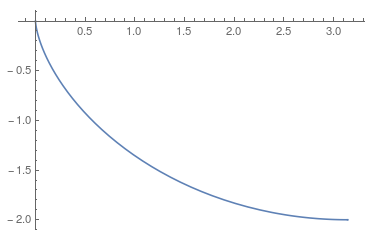
\includegraphics[scale=0.5]{img/cicloide.png}
  \caption{Ejemplo de cicloide}
\end{figure}

\section{Relación de ejercicios}

\begin{ejercicio}
Encontrar la curva en la que el siguiente funcional podría alcanzar su extremo:
\[
I(y)=\integral{1}{2}{\Big(y'(x)^2-2xy(x)\Big)dx}
\]
con condiciones de contorno $y(1)=0,y(2)=-1$.
\end{ejercicio}
\textbf{Solución:}
Definimos $F(x,y,p)=p^2-2xy$ y obtenemos:
\[
\derivada{F}{p}=2p, \espacio \derivada{F}{y}=-2x \Rightarrow Z(x)=2y'(x), \espacio Z'(x)=-2x
\]
Resolviendo la ultima ecuación, obteniendo:
\[
Z(x)=-x^2+C \Rightarrow 2y'(x)=-x^2+C \Rightarrow y'(x)=\frac{-x^2+C}{2}\Rightarrow y(x)=-\frac{x^3}{6}+\frac{c}{2}x+D
\]
Usando las condiciones de contorno, podemos calcular el valor de $C$ y $D$, obteniendo:
\[
y(x)=\frac{x-x^3}{6}
\]
\begin{ejercicio}
Encuentra las curvas que unen $(1,3)$ con $(2,5)$, que puedan ser extremos del funcional:
\[
I(y)=\integral{1}{2}{\Big(y'(x)+x^2y'(x)^2\Big)dx}
\]
\end{ejercicio}

\textbf{Solución} $y(x)=-\frac{4}{x}+7$

\begin{ejercicio}
  Sean $\Phi\in \mathcal{C}^1(\mathbb{R}^3), y(x)\in \mathcal{C}^2\xcero, y'(x) \neq 0$. Dado el funcional
  \[
    F[y] = \int_{a}^{b}{\Phi(x,y(x),y'(x))dx}
  \]
  demuéstrese la equivalencia de las dos formas siguientes de las
  ecuaciones de Euler-Lagrange.
  \begin{itemize}
  \item[$a)$] $\frac{\partial\Phi}{\partial y}-\frac{d}{dx}\frac{\partial\Phi}{\partial p} = 0 $
  \item[$b)$] $\frac{\partial\Phi}{\partial x} - \frac{d}{dx}(\Phi-y'\frac{\partial\Phi}{\partial p}) = 0$
  \end{itemize}
  \begin{proof}
    Comenzamos viendo el caso $a) \implies b)$. Del apartado $a)$ sabemos que
    \[
      \frac{\partial\Phi}{\partial y} = \frac{d}{dx}\frac{\partial\Phi}{\partial p}
    \]
    y del enunciado sabemos que $\Phi$ es de calse $\mathcal{C}^1$
    luego $\frac{\partial\Phi}{\partial p}$ es de $\mathcal{C}^1$.

    Cuando derivamos $\Phi(x,y(x),y'(x))$ obtenemos
    \begin{align*}
      \frac{d\Phi}{dx}(x,y(x),y'(x)) & = \frac{\partial\Phi}{\partial x}(x, y(x), y'(x)) \\
                          & + \frac{\partial\Phi}{\partial y}(x, y(x), y'(x))y'(x) \\
                          & + \frac{\partial\Phi}{\partial p}(x, y(x), y'(x))y''(x)
    \end{align*}
    Recordemos que $\frac{\partial\Phi}{\partial p}(x, y(x), y'(x)) = z(x)$ luego
    \begin{align*}
      \frac{d}{dx}(\Phi-y'\frac{\partial\Phi}{\partial p}) & = \Phi_x + \Phi_yy' + \Phi_py'' - y''z -y'z'
    \end{align*}
    Tenemos que el 3º y 4º termino son opuestos, al igual que el 2º y 5º, luego obtenemos
        \begin{align*}
      \frac{d}{dx}(\Phi-y'\frac{\partial\Phi}{\partial p}) = \Phi_x
        \end{align*}

        que es lo que queríamos.

        $b)\implies a)$
        
        Todos los pasos que hemos dado son reversibles pero
        necesitamos ver que
        $\frac{\partial\Phi}{\partial p}(x, y(x), y'(x))$ es $\mathcal{C}^1$.

        Llamando $H(x) = \Phi-y'(x)z(x)$, por hipótesis tenemos que
        $H$ es derivable. Despejando tenemos que

        \[
          z = \frac{\Phi-H}{y'}
        \]

        luego $z$ es derivable por ser cociente de derivables ($y'\neq 0$).

        \begin{align*}
          \Phi_x & = \Phi_x + \Phi_yy' + \Phi_py'' - y''z -y'z' \\
                 & \implies y'(\Phi_y-z') = 0
        \end{align*}

        e $y' \neq 0$ por hipótesis, luego $\Phi_y - z' = 0$.
  \end{proof}
\end{ejercicio}
\begin{ejercicio}
Obténgase la forma que adopta la ecuación de Euler-Lagrange en los siguientes casos particulares:

\begin{enumerate}[a)]
\item $\Phi$ sólo depende de $y'$.
    \begin{proof}
      Usando el apartado a) del ejercicio anterior y sustituyendo $\frac{\partial\Phi}{\partial y}=0$ obtenemos
      \[
        \frac{d}{dx}\Phi_p = 0
      \]

      De donde deducimos que $\Phi_p(y'(x))$ es una constante.
    \end{proof}
\item $\Phi$ no depende de $y$.
\item $\Phi$ no depende explícitamente de $x$.
\item $\Phi=G(x,y)\sqrt{1+y'^2}$.
\end{enumerate}
\end{ejercicio}

\begin{ejercicio}
Aplíquense los resultados anteriores a los ejemplos siguientes:
\begin{enumerate}[a)]
\item $\mathcal{F}(y(x))=\integral{}{}{y(2x-y)dx}$, $y(0)=0$, $y(\pi/2)=\pi/2$.
\item $\mathcal{F}[y(x)] =\integral{}{}{y(2x-y)dx}, \quad y(0) = 0, \quad y(\pi/2) = \pi/2$

    Definimos $F(x,y,p) = y(2x-y)$. Se cumple

    \begin{align*}
      F_p &= 0\\
      z(x) &= 0\\
      F_y(x,y(x)) &= 2y(x)-2x
    \end{align*}

    De aquí obtenemos $2x-2y = 0 \implies y(x) = x$. Ahora tenemos que
    comprobar que la solución cumple las condiciones de contorno.

    \[
      y(0) = 0, \quad y(\pi/2) = \pi/2
    \]
    
    Luego se cumplen ambas condiciones.
\item $\mathcal{F}(y(x))=\integral{}{}{(y^2+2xyy')dx}$, $y(a)=A$, $y(b)=B$.
\item $\mathcal{F}(y(x))=\integral{}{}{y'(1+x^2y')dx}$, $y(1)=3$, $y(2)=5$.
\end{enumerate}
\end{ejercicio}

 
%\chapter{Derivadas débiles}

Recordemos el espacio $L^1(a,b)$ de las funciones $\funcion{f}{(a,b)}{\R}$ que son Lebesgue integrables. Ese espacio estaba formado por clases de equivalencia, que normalmente llamamos clases de funciones. Que sea Lebesgue integrable, no quiere decir que sea continua, como nos indica la \textit{función de Dirichlet}, que es Lebesgue integrable pero evidentemente no es continua.
\[
f(x)=\left\{
\begin{array}{cc}
0 & x\notin\mathbb{Q} \\
1 & x\in\mathbb{Q}
\end{array}
\right. 
\]
Toda función continua no es integrable, necesitamos que esté acotada. Eso nos dice que todas las funciones continuas no están en $L^1(a,b)$. Para evitar eso, definimos el \textit{espacio de funciones continuas localmente integrables}, que denotaremos por:
\[
L^1_{loc}(a,b)=\{\funcion{f}{(a,b)}{\R} \;|\; \forall J \text{ intervalo compacto},f_{|J}\text{ es integrable}\}
\]
Ese espacio soluciona el problema anterior ya que todas las funciones continuas sí son localmente integrables. Solucionado el problema, podemos definir la derivada débil con tranquilidad:

\begin{definition}
Sean $f,g\in\localmenteintegrable$, se dice que $g$ es la derivada débil de $f$ si se verifica que:
\[
\integral{a}{b}{f\phi'}+\integral{a}{b}{g\phi}=0 \espacio \forall\phi\in\soportecompacto
\]
\end{definition}

Cabe resaltar, que la definición anterior implica que la derivada débil de una función no es única, es decir, una función $f$ puede admitir varias derivadas débiles. Sin embargo, como veremos en el siguiente corolario, serán iguales para casi todo punto.

\section{Propiedades básicas}

Podemos generalizar el lema fundamental del cálculo de variciones:

\begin{theorem}
Si $f\in\localmenteintegrable$ cumpliendo:
\[
\integral{a}{b}{f(x)\phi(x)dx}=0 \espacio\forall\phi\in\soportecompacto
\]
Entonces $f(x)=0$ $a.e$ $x\in(a,b)$.
\end{theorem}
Este resultado engloba al visto previamente en el teorema \ref{theorem:1.3}. Como consecuencia, tenemos:
\begin{coro}
Sea $f\in\localmenteintegrable$ y $g,\tilde{g}\in\localmenteintegrable$ dos derivadas débiles de $f$. Entonces $g(x)=\tilde{g}(x)$ $a.e$ $x\in(a,b)$.
\end{coro}

\begin{proof}
Simplemente usando la definición y el lema generalizado tenemos:
\[
\left.
\begin{array}{c}
\integral{a}{b}{f\phi'}+\integral{a}{b}{g\phi}=0 \\
\integral{a}{b}{f\phi'}+\integral{a}{b}{\tilde{g}\phi}=0
\end{array}
\right\} \Rightarrow \integral{a}{b}{(g-\tilde{g})\phi}=0 \Rightarrow g=\tilde{g} \; a.e
\]
\end{proof}

Para la demostración del lema generalizado, necesitaremos algunas herramientos previas. Recordemos primeramente una propiedad de las funciones Lebesgue integrables:

\begin{prop}
Dado $f\in\localmenteintegrable$, existe una secuencia de funciones simples, $\{g_n\}$, tal que $\{g_n\}\longrightarrow f$.
\end{prop}

\begin{lemma}
Sea $g$ una función simple, entonces existe una sucesión de funciones de soporte compacto $\phi_n\in\soportecompacto$ tal que $\{\phi_n\}\longrightarrow g \; a.e$ y además $|\phi_n(x)|\leq|g(x)|$.
\end{lemma}

Ahora ya sí podemos demostrar el lema generalizado:

\begin{proof}
Sea $g$ una función simple. Por el lema anterior, puedo tomar una sucesión $\phi_n$ de funciones de soporte compacto convergiendo a $g$.Usando el teorema de la convergencia dominada de Lebesgue, podemos intercambiar el límite en la siguiente integral:
\[
\limitemasinfinito{n}{\integral{}{}{\phi_n(x)f(x)dx}}=\integral{}{}{g(x)f(x)}dx
\]
Por la proposición anterior, nos podemos tomar una sucesión $g_n$ de funciones simples de forma que $\{g_n\}\longrightarrow f \; a.e$. De forma análoga:
\[
0=\limitemasinfinito{n}{\integral{}{}{g_n(x)f(x)dx}}=\integral{}{}{f(x)^2}dx \Rightarrow f\equiv 0 \; a.e
\]
\end{proof}

La derivada débil tiene una propiedad parecida a la derivada clásica, ambas son conceptos locales, es decir:

\begin{prop}
Si $f$ es una función que admite derivada débil $f'=g$ en $(a,b)$, y tomamos $(a',b')\subset(a,b)$, entonces $f_{|(a',b')}$ admite derivada débil y vale $g_{|(a',b')}$.
\end{prop}

\begin{proof}
Evidente usando el hecho de que $\mathcal{D}(a',b')\hookrightarrow\soportecompacto$.
\end{proof}

Toda función derivable no es derivable débil, como ilustra el siguiente ejemplo:

\begin{example}
La función $\funcion{f}{\R}{\R}$ definida por $f(x)=\sqrt{|x|}$, es derivable débil pero no derivable.

Primero tenemos que ver que $g\in\localmenteintegrable$. Si el intervalo compacto $J$ escogido no contiene al 0, entonces podemos integral sin problema. En caso contrario, tenemos que ver qué pasa con la siguiente integral:
\[
\integral{-\varepsilon}{\varepsilon}{|g(x)|dx}\overset{g\; simetrica}{=}2\integral{0}{\varepsilon}{|g(x)|dx}=2\integral{0}{\varepsilon}{\frac{1}{2\sqrt{x}}}=2\sqrt{x}\Big|_0^\varepsilon=2\sqrt{\varepsilon}<+\infty
\]
Ahora tenemos que comprobar que $g$ es la derivada débil de $f$, es decir:
\[
\integral{\R}{}{f\phi'}+\integral{\R}{}{g\phi}=0 \espacio \forall\phi\in\soportecompacto
\]
\[
\integral{\R}{}{f(x)\phi'(x)dx}=\integral{|x|>\varepsilon}{}{f(x)\phi'(x)dx}+\underbrace{\integral{|x|<\varepsilon}{}{f(x)\phi'(x)dx}}_{f\phi'\leq2\sqrt{\varepsilon}\max\phi'\to0}=\integral{|x|>\varepsilon}{}{f(x)\phi'(x)dx}=
\]
\[
=\integral{-\infty}{-\varepsilon}{f(x)\phi'(x)dx}+\integral{\varepsilon}{+\infty}{f(x)\phi'(x)dx}=
\]
\[
=\underbrace{f(x)\phi(x)\Big|_{-\infty}^{-\varepsilon}}_{=f(-\varepsilon)\phi(-\varepsilon)\to 0}-
\integral{-\infty}{-\varepsilon}{g(x)\phi(x) dx}+
\underbrace{f\phi\Big|_{\varepsilon}^{+\infty}}_{{=f(\varepsilon)\phi(\varepsilon)\to 0}}-
\integral{\varepsilon}{+\infty}{g(x)\phi(x) dx}=
\]
\[
-\integral{\R}{}{g(x)\phi(x)dx}+\underbrace{\integral{|x|<\varepsilon}{}{g(x)\phi(x)dx}}_{\to0}=-\integral{\R}{}{g(x)\phi(x)dx}
\]
\end{example}

Vamos a ver que la derivada de una integral de una derivada débil, es la propia función (como es de esperar). Para ello vamos a tener que desarrollar una serie de pasos previos.

\begin{theorem}
\label{fundamentalcalculo}
Sea $g\in\localmenteintegrable$ y tomo $x_0\in(a,b)$. Defino $\funcion{f}{(a,b)}{\R}$ como
\[
f(x)=\integral{x_0}{x}{g(x)ds}
\]
Entonces $f'=g$ y $f\in C[a,b]$.
\end{theorem}

\begin{proof}

La integral en $f$ tiene sentido ya que $[x_0,x]\subset (a,b)$. Comprobemos que $f\in C(a,b)$. Tomamos $\{x_n\}$ sucesión de puntos de $(x_0,x)$ tal que $x_n\to \tilde{x}\in[x_0,x]$ (por ser compacto).

\begin{center}

\begin{tikzpicture}[scale=0.5]
\draw (-1,0)-- (9,0); %Axis

\draw (0,-.5) -- (0,.5);
\draw (0,-0.5) node[anchor=north] {$a$};

\draw [thick] (2.1,-.5) -- (2,-.5) -- (2,.5) -- (2.1,.5); 
\draw (2,-.5) node [anchor=north] {$x_0$};

\draw (3.5,-.5) -- (3.5,.5);
\draw (3.5,-0.5) node[anchor=north] {$x_n$};

\draw (4.5,-.5) -- (4.5,.5);
\draw (4.5,-0.5) node[anchor=north] {$\tilde{x}$};

\draw [thick] (6,-.5) -- (6.1,-.5) -- (6.1,.5) -- (6,.5); 
\draw (6,-.5) node [anchor=north] {$x$};

\draw (8,-.5) -- (8,.5);
\draw (8,-0.5) node[anchor=north] {$b$};

\end{tikzpicture}
\end{center}

\begin{enumerate}[-]
\item Si $x\notin[x_0,\tilde{x}] \Rightarrow x\notin [x_0,x_n]$ para $n\geq n_0$.
\item Si $x\in(x_0,\tilde{x}) \Rightarrow x\in [x_0,x_n]$ para $n\geq n_0$.
\end{enumerate}

Y ese es la clave que nos va a permitir ver que $f(x_n)\to f(\tilde{x})$. Sea $J$ un intervalo compacto de forma que $[x_0,x]\subset J\subset(a,b)$.
\[
\integral{x_0}{x_n}{g(x)dx}=\integral{J}{}{g(x)\chi_{[x_0,x_n]}}(x)dx
\]
Usando lo anterior obtenemos la convergencia puntual de la sucesión $g(x)\chi_{[x_0,x_n]}\overset{cp}{\longrightarrow}g(x)\chi_{(x_0,\tilde{x})}$. Lo que nos da la convergencia en integral también:
\[
f(x_n)=\integral{J}{}{g(x)\chi_{[x_0,x_n]}(x)dx}\overset{cp}{\longrightarrow}\integral{J}{}{g(x)\chi_{(x_0,\tilde{x})}(x)dx}=\integral{x_0}{\tilde{x}}{g(x)dx}=f(\tilde{x})
\]
Luego $f\in C(a,b) \Rightarrow f\in \localmenteintegrable$.
Ahora nos queda ver $f'=g$. Para ello tenemos que comprobar que:
\[
\integral{a}{b}{f(x)\phi'(x)dx}+\integral{a}{b}{g(x)\phi(x)dx}=0 \espacio \forall \phi\in \soportecompacto
\]
Tenemos el problema de que $g$ no tiene por qué ser derivable (podría ser una función escalón, por ejemplo). Vamos a empezar suponiendo que $g\in L^1([a,b])$ (para que $f$ esté bien definida) y que $x_0=a$. Al final reduciremos esas hipótesis hasta llegar a que $g\in\localmenteintegrable$.

\underline{Paso 1}: $g\in L^1([a,b])$ y $x_0=a$. Para ver que
\[
\integral{a}{b}{f(x)\phi'(x)dx}=-\integral{a}{b}{g(x)\phi(x)dx} 
\]
vamos a tener que usar el Teorema de Fubini-Tonelli.
\[
\integral{a}{b}{f(x)\phi'(x)dx}=
\integral{a}{b}{\left(\integral{a}{x}{g(s)ds}\right)\phi'(x)dx}\overset{TªFT}{=}
\integral{a}{b}{\left(\integral{s}{b}{g(s)\phi'(x)dx}\right)ds}=\]
\[
\integral{a}{b}{g(s)\left(\integral{s}{b}{\phi'(x)dx}\right)ds}
=\integral{a}{b}{g(s)(\underbrace{\phi(b)}_{=0}-\phi(s))ds}=-\integral{a}{b}{g(s)\phi'(s)ds}
\]
\underline{Paso 2}: Reemplazamos la hipótesis $x_0=a$ por $x_0\in(a,b)$ y usamos el paso 1:
\[
\integral{a}{b}{g(x)\phi(x)dx}=-\integral{a}{b}{\left(\integral{a}{x}{g(s)ds}\right)\phi'(x)dx}
\]
Vemos que la integral del interior se puede expresar como una constante más una función:
\[
\integral{a}{x}{g(s)ds}=\underbrace{\integral{a}{x_0}{g(s)ds}}_{cte=C}+\underbrace{\integral{x_0}{x}{g(s)ds}}_{funcion}
\]
Luego:
\[
-\integral{a}{b}{\left(\integral{a}{x}{g(s)ds}\right)\phi'(x)dx}=
-\underbrace{\integral{a}{b}{B\phi'(x)dx}}_{=B(\phi(b)-\phi(a))=0}-\integral{a}{b}{\left(\integral{x_0}{x}{g(s)ds}\right)\phi'(x)dx}=
-\integral{a}{b}{f(x)\phi(x)dx}
\]
\underline{Paso 3}: Ahora sustituimos la hipótesis $g\in L^1([a,b])$ por $g\in\localmenteintegrable$. Tomamos un subintervalo compacto $[a'.b']\subset(a,b)$ donde $g_{|[a'.b']}\in L^1([a',b'])$, de forma que $\supp\phi\subset[a',b']$. Sea $x_0\in[a',b']$ y $x\in(a,b)$.

Ahora aplicamos el caso 2, usando que $\supp\phi\subset[a',b']$:
\[
\integral{a}{b}{g(x)\phi(x)dx}=\integral{a'}{b'}{g(x)\phi(x)dx}=-\integral{a'}{b'}{\left(\integral{x_0}{x}{g(s)ds}\right)\phi'(x)dx}=-\integral{a}{b}{f(x)\phi'(x)dx}
\]
\end{proof}

Una vez obtenida una versión para derivadas débiles del Teorema Fundamental del Cálculo, vamos a ver más propiedades de este concepto.

La siguiente proposición nos permitirá obtener un representante continuo a partir de una función que tenga derivada débil, pero no tengo por qué ser continua.

\begin{prop}
\label{representantecontinuo}
Si $f\in\localmenteintegrable$ tiene derivada débil en $(a,b)$, entonces existe $\tilde{f}\in C(a,b)$ tal que $\tilde{f}(x)=f(x)$ $a.e$ $x\in(a,b)$.
\end{prop}

\begin{proof}
Sea $f\in\localmenteintegrable$, $\funcion{g}{(a,b)}{\R}$ su derivda débil, es decir, $f'=g$ y $x_0\in(a,b)$. Definimos $\funcion{\tilde{f}}{(a,b)}{\R}$ por:
\[
\tilde{f}(x)=\integral{x_0}{x}{g(s)ds}
\]
El resultado anterior nos da que $\tilde{f}\in C(a,b)$ y $\tilde{f}'=g$. Solo nos falta ver que $\tilde{f}$ es igual casi por doquier a $f$, o lo que es lo mismo, comprobar que $f-\tilde{f}$ tiene derivada débil 0:
\[
\left.
\begin{array}{cc}
\integral{a}{b}{f(x)\phi'(x)dx}=-\integral{a}{b}{g(x)dx} \\
\integral{a}{b}{\tilde{f}(x)\phi'(x)dx}=-\integral{a}{b}{g(x)dx}
\end{array}
\right\} \Rightarrow \integral{a}{b}{(f-\tilde{f})(x)\phi'(x)}=-\integral{a}{b}{0\phi(x)dx}
\]
\end{proof}

\begin{prop}
\label{derivadadebilcero}
Si $f\in\localmenteintegrable$ y tiene derivada débil igual a 0, entonces $f$ es constante $\casipordoquier$.
\end{prop}

\begin{proof}
La demostración de este es prácticamente igual a la demostración del Lema \ref{lemma:14}.
\end{proof}

\begin{example}[examen 18/19]
Sea $\funcion{f}{\R\backslash\{1\}}{\R}$ definida por $f(x)=\frac{(x-1)(x+2)}{|x-1|}$. ¿Tiene derivada débil?

Nos damos cuenta de que $f(x)=\frac{(x-1)(x+2)}{|x-1|}=\frac{x-1}{|x-1}(x+2)$, es decir, $f$ se expresa como producto de una función escalón (discontinua), por un polinomio (continuo), luego $f$ es discontinua.

Como es discontinua, si tuviera derivada débil, por la proposición \ref{representantecontinuo} , debe existir $\tilde{f}$ función continua tal que $f(x)=\tilde{f}(x)\;\; a.e$. Veamos que esa función no puede existir. El conjunto $\{x:\;\; f(x)=\tilde{f}(x)\}$ tiene \textbf{medida llena} (complementario con medida nula), luego es denso. Tomamos $\{x_n\}\longrightarrow 1$ y vemos que:
\[
3=\limite{n}{1^+}{f(x_n)}=\limite{n}{1^+}{\tilde{f}(x_n)}
\]
\[
-3=\limite{n}{1^-}{f(x_n)}=\limite{n}{1^-}{\tilde{f}(x_n)}
\]
Pero $\tilde{f}$ es continua, luego esos límites deberían coincidir: contradicción.

\end{example}

\begin{prop}
\label{derivadanesima}
Sea $f\in\localmenteintegrable$ $n$-veces derivable débil, entonces existe $\tilde{f}$ tal que $f(x)=\tilde{f}(x) \; \casipordoquier$ y además $\tilde{f}\in C^{n-1}(a,b)$.
\end{prop}

\begin{proof}
\underline{Caso n=1}: Si $f$ tiene derivada débil, sabemos por la proposición \ref{representantecontinuo} que existe $\tilde{f}\in C(a,b)$ y $f(x)=\tilde{f}(x) \;\casipordoquier$.
El caso $n$ se deduce fácilmente del siguiente hecho:
\[
\left.
\begin{array}{r}
\integral{a}{b}{\tilde{f}(x)\phi'(x)dx}+\integral{a}{b}{g(x)\phi(x)dx}=0 \\
\tilde{f}, g \text{ continuas }
\end{array}
\right\} \Rightarrow \tilde{f}\in C^1(a,b), \;\tilde{f}'=g \text{ (en sentido clásico)}
\]
\underline{Caso n}: Suponemos que $f$ es $(n-1)$-veces derivable débil y que existe $\tilde{f}\in C^{n-2}(a,b)$ tal que $f(x)=\tilde{f}(x)\;\casipordoquier$.
Si derivamos $(n-1)$-veces $f$, obtenemos $\tilde{f}^{n-1)}=f^{n-1)}=g$, que no sabemos si es continua, pero sabemos que podemos elegir un representante que si lo sea. Usando el hecho anterior, tenemos que $\tilde{f}\in C^{n-1}(a,b)$.
\end{proof}

\section{The Devil Staircase}

Nuestro objetivo va a ser construir una función continua$\funcion{f}{\R}{\R}$ que no admita derivada débil.

En $\R\backslash(0,1)$ será constante:
\[
f(x)=\left\{
\begin{array}{cc}
0 & x\leq 0\\
1 & x\geq 1
\end{array}
\right.
\]
En $(0,1)$ nos va a costar un poco más construirla. Para ello, definimos primeramente \textit{el conjunto ternario de Cantor}, que se construye sobre el intervalo $[0,1]$, eliminando en cada paso el segmento abierto correspondiente al tercio central de cada intervalo.

\begin{figure}[h]
   \center
  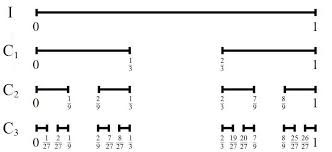
\includegraphics[scale=0.5]{img/cantor.jpeg}
  \caption{Representación gráfica}
\end{figure}

Es fácil ver que la media del primer conjunto $C_0$ es $2/3$, el de $C_1$ $4/9$, y el de $C_n=(\frac{2}{3})^n$. Además, cada $C_n$ es compacto, luego si consideramos como conjunto $C$ a la intersección de todos, es decir, $C=\cap_{n\in\N} C_n$, obtenemos otro conjunto compacto. $C$ tiene media nula, ya que $\mu(C)=\left(\frac{2}{3}\right)^n\to0$.

Vamos a construir nuestra $f$ sobre el complementario de ese conjunto, es decir, sobre $B=(0,1)\backslash C$.

Nuestra función será constante en cada intervalo de $B$, es decir, en los intervalos que hemos sustraído al construir el conjunto ternario de Cantor. Para hacerla continua, necesitamos regularizar cada salto entre intervalos, definiendo $f$ en esa parte como una recta que conecte cada intervalo con el siguiente.

\begin{figure}[H]
   \center
  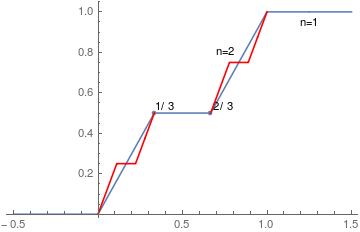
\includegraphics[scale=0.6]{img/escalera.png}
\end{figure}

Denotamos por $f_n$ a la función resultante de realizar el paso anterior $n$ veces, consiguiéndo así una sucesión de funciones continuas. Esta sucesión cumple además una propiedad clave para nosotros: si $x\in B$, existe un $n_0\in\N$ tal que si $n\geq n_0$, entonces $x$, debe de estar en algún intervalo, $I_{n_0}$. Pero en esos intervalos, que son los eliminados por el conjunto de Cantor, nuestra función es constante, es decir, $f_n$ es constante en $I_{n_0}$.

Una vez realiza esta construcción, podemos definir nuestra función $f$ como sigue:
\[
f(x)=\limitemasinfinito{n}{f_n(x)}
\]
Tenemos que ver que $f_n$ converge para que la definición de $f$ tenga sentido. Debido a la forma en la que hemos construido la sucesión $f_n$, tenemos que:

\begin{figure}[H]
   \center
  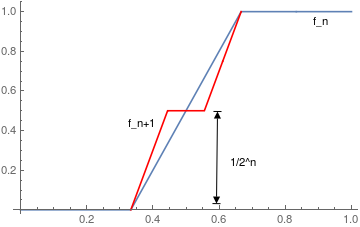
\includegraphics[scale=0.6]{img/convergenciaescalera.png}
\end{figure}
\[
\valorabsoluto{f_n(x)-f_{n+1}(x)}\leq\frac{1}{2^n} \Rightarrow \norm{f_n(x)-f_{n+1}}_{\infty}\leq \frac{1}{2^n}
\]

Expresando ahora $f_n$ usando la forma telescópica de una sucesión:
\[
f_n(x)=f_1(x)+f_2(x)-f_1(x)+...=f_1(x)+\sum_{n=1}^\infty\left(f_{n+1}(x)-f_n(x)\right) \Rightarrow \norm{f_n}_{\infty}\leq \frac{1}{2^n}
\]
Obteniendo así que $f_n$ converge uniformemente a $f$, y como $f_n$ es continua para todo $n\in\N$, $f$ también lo es. 

Ya tenemos nuestra \textit{escalera continua} construida, falta ver que no tiene derivada débil. Supongamos que existe $g$ tal que $f'=g$. Como $f$ está definida como una función constante en cada componente conexa de $B$, su derivada vale 0, es decir, $g(x)=0\;$ si $x \in B$ o $x\leq 1$ o $x\leq 0$. Pero, como $B$ tiene medida llena, lo anterior implica que $g(x)=0 \; a.e \; x\in\R$, luego $f$ sería constante, lo cual es una evidente contradicción.

%\chapter{Espacios de Sobolev}

A lo largo de los temas 1 y 2, hemos construido una serie de herramientas básicas en la resolución de ciertos modelos matemáticos. A continuación, vamos a enlazar los conceptos vistos anteriormente y desarrollar los primeros modelos de esta asignatura.

\section{Enlace}

Antes de definir los \textit{espacios de Sobolev}, recordemos algunas propiedades del espacio 
\[L^2(a,b)=\displaystyle\{\funcion{f}{(a,b)}{\R}\;:\; \integral{a}{b}{|f(x)|^2dx<+\infty}\displaystyle\}\]
La norma de este espacio venía dada por $\norm{f}_2=\sqrt{\integral{a}{b}{f(x)^2dx}}$ e inducía el siguiente producto escalar: $<f,g>=\integral{a}{b}{f(x)g(x)dx}$ (nótese que no usamos el conjugado de $g$ ya que estamos trabajando sobre $\R$, no sobre $\C$). Además, $L^2(a,b)\subset L^1(a,b)$ ya que 
\[
\integral{a}{b}{f(x)}=\integral{a}{b}{|f(x)|\cdot 1dx}\leq \left(\integral{a}{b}{f(x)^2dx}\right)^{1/2}\left(b-a\right)^{1/2}
\]
donde hemos usado la desigualdad de Schwartz para el último paso. Con estas propiedades en mente, podemos definir el primer espacio de Sobolev:
\[
\sobolev{1}=\conjunto{f\in\lebesgue{2}: f \text{ tiene derivada débil }f' \text{ y } f'\in\lebesgue{2}}
\]
Este espacio tiene la particularidad de que también cuenta con un producto escalar:
\[
<f,g>=\integral{a}{b}{f(x)g(x)dx}+\integral{a}{b}{f'(x)g'(x)dx}
\]
Por supuesto, $\sobolev{1}$ es un espacio de Hilbert con la norma $\norm{f}=\sqrt{\norm{f}^2_2+\norm{f'}_2^2}$. Es importante recordar que si $f\in\sobolev{1}$, no tiene por qué ser continua (como muestra \textit{The devil staircase}), pero podemos elegir un representante continuo en su clase de equivalencia, es decir, $\sobolev{1}\hookrightarrow C[a,b]$. De hecho:
\begin{prop}\label{inclusion continua}
La aplicación inclusión $\funcion{i}{\sobolev{1}}{C[a,b]}$ es continua.
\end{prop}
\begin{proof}
Pendiente.
\end{proof}
Además, si $f\in C^1[a,b]$, tiene derivada clásica, luego también tiene derivada débil, luego $f\in\sobolev{1}$. Resumiendo, hemos construido la siguiente cadena:
\[
C^1[a,b]\subset\sobolev{^1}\subset C[a,b]\subset \lebesgue{2}
\]
Definimos ahora el siguiente espacio de Sobolev:
\[
\sobolev{2}=\conjunto{f\in\lebesgue{2}: \exists f',f''\in\lebesgue{2}\text{ (débiles)}}
\]
Usando la propiedad \ref{derivadanesima}, tenemos que $\sobolev{2}\subset C^1[a,b]$ y repitiendo el argumento anterior $C^2[a,b]\subset \sobolev{2}$, es decir:
\[
C^2[a,b]\subset \sobolev{2}\subset C^1[a,b]
\]
Repitiendo este proceso iterativamente, podemos definir el $n$-ésimo espacio de Sobolev:
\[
\sobolev{n}=\conjunto{f\in\lebesgue{2}: \exists f',\dots,f^{n)}\in\lebesgue{2} \text{ (débiles)}}
\]
con la propiedad:
\[
C^{n}[a,b]\subset\sobolev{n}\subset C^{n-1}[a,b]\subset\sobolev{n-1}\subset\dots\subset\sobolev{1}\subset\lebesgue{2}
\]

¿Qué tienen de particular estos espacios? Que son de Hilbert, es decir, vamos a poder usar todas las herramientes que tenemos de Análisis Funcional para resolver algunos problemas como veremos en los siguientes apartados.

\begin{definition}
Diremos que $\funcion{F}{[a,b]\times\R^2}{\R}$ es una \textit{función de Carathéodory} si cumple:
\begin{enumerate}[(a)]
\item Para casi todo punto $x\in(a,b)$, $F(x,y,p)$ es continua en $(y,p)$.
\item Para casi todo punto $(y,p)\in\R^2$, la función $x\mapsto F(x,y,p)$ es medible.
\item Dado $K\subset[a,b]\times\R^2$ compacto, existe una función $m_k(x)\in\lebesgue{1}$ tal que $\valorabsoluto{F(x,y,p)}\leq m_k(x)$ $\forall(x,y,p)\in K$.
\end{enumerate}
\end{definition}

Para que la teoría que vamos a desarrollar a continuación tenga sentido, vamos a imponer de ahora en adelante que $F$, $F_y$ y $F_p$ sean de Carathéodory. Haciendo uso de la propiedad (c), podemos definir el funcional $\funcion{L}{\sobolev{1}}{\R}$:
\[
L(y)=\integral{a}{b}{F(x,y(x),y'(x))dx}
\]
que está bien definido ya que que $F$ es medible y está acotada por una función que es integrable. Tomando $\phi\in\soportecompacto$, podemos definir otra función $\funcion{g}{[a,b]}{\R}$ por $g(s)=L(y+s\phi)$, derivarla respecto a $s$ y evaluarla en 0 (a esta expresión la llamamos \textit{derivada de y a lo largo de $\phi$}):
\[
g'(0)=DL_y(\phi)=\integral{a}{b}{F_y(x,y(x),y'(x)dx}+\integral{a}{b}{F_p(x,y(x),y'(x)dx}
\]
\newpage

\section{Modelos de cuerdas}

Procedemos a la introducción del \textit{modelo de cuerdas}. Comenzaremos realizando el planteamiento más simple, densidad constante y extremos fijos. Posteriormente, eliminaremos la primera hipótesis y resolveremos dos casos: en el primero partimos de una función de densidad dada explícitamente. Por el contrario, en el segundo caso, lo resolveremos dada una función de densidad arbitraria. A continuación, supondremos que el puente se haya \textit{sujeto} por varias cuerdas elásticas. Finalmente, supondremos fijos los extremos.

Aunque ya hemos desarrollado una cantidad de resultados considerable, todavía precisamos de ciertos resultados, mayoritariamente del \textit{Análisis Funcional}, que iremos introduciendo al mismo tiempo que el modelo. Como estamos trabajando sobre espacios de Sobolev, que son de Hilbert, podremos usarlos sin mucha complicación.

\subsection{Extremos fijos y densidad constante}

Supongamos tener una \textit{cuerda elástica}, colgada entre dos puntos, 0 y 1, es decir, nuestra cuerda está representada por una función $\funcion{y}{[0,1]}{\R}$ en $\sobolev{1}$ tal que $y(0)=y(1)=1$. El objetivo del modelo será encontrar la \textit{cuerda} de mínima energía. En este caso, vamos a suponer que la \textit{densidad} de la cuerda es una constante $m\in\R^+$. 

Denotamos por $E_p$ a la energía potencial y por $E_e$ a la energía elástica:
\[
E_e=\frac{1}{2}\integral{0}{1}{y'(x)^2dx} \espacio\espacio E_p=\integral{0}{1}{my(x)dx}
\]
Minimizar la energía total de la cuerda, es lo mismo que minimizar el funcional:
\[
L(y)=\frac{1}{2}\integral{0}{1}{y'(x)^2dx}+\integral{0}{1}{my(x)dx}
\]
Usando la notación usual:
\[
L(y)=\integral{0}{1}{F(x,y,p)dx} \; \text{ donde } \;\; F(x,y,p)=\frac{1}{2}p^2+my
\]
Supongamos que $y\in\sobolev{1}$ es un punto crítico del funcional $L:\sobolev{1}\longrightarrow\R$ para poder usar la teoría de la \textit{ecuación de Euler}.
Si calculamos las derivadas parciales de $F(x,y,p)$:
\[
Z(x)=F_p(x,y,p)=p=y'(x) \espacio Z'(x)=F_y(x,y,p)=m
\]
vemos que $Z(x)$ tiene derivada débil ($Z'(x)$), como consecuencia, $y'(x)$ es continua (proposición \ref{representantecontinuo}). Pero además, $Z'(x)=(y'(x))'=y''(x)=m$, continua, por lo tanto $y\in C^2[0,1]$. En resumen, tenemos que resolver la siguiente EDO de segundo orden:
\[
\left\{
\begin{array}{rl}
y''(x) & = m \\
y(0) & = 0 \\
y(1) & = 0
\end{array}
\right.
\]
Si recordamos algo de ecuaciones diferenciales, nos damos cuenta de que las condiciones iniciales están \textit{mal planteadas}. Para poder resolver la ecuación, necesitamos dos conciones sobre el mismo punto: una en $y$ y otra en $y'$. Lo podemos solucionar usando el llamado \textit{método de tiro}, que consiste en darle un valor arbitrario a la condición que nos falta, resolver la ecuación y despejar el valor posteriormente. Asumiendo que $y'(0)=\alpha\in\R$, nos queda:
\[
\left\{
\begin{array}{rl}
y''(x) & = m \\
y'(0) & = \alpha \\
y(0) & = 0
\end{array}
\right.
\]
con solución $y(x)=\integral{0}{x}{\left(\alpha+msds\right)}=m\frac{x^2}{2}+\alpha x$. Usando $y(1)=0$, obtenemos que $\alpha=-\frac{m}{2}$. Por lo que la solución del modelo es:
\[
y(x)=\frac{m}{2}x(x-1) \;\; \forall x \in[0,1]
\] 

\subsection{Extremos fijos y densidad no constante}

El planteamiento es igual al anterior, pero suponemos que la densidad en lugar de ser constante es la función $\funcion{q}{[0,1]}{\R}$ dada por:
\[
q(x)=\left\{\begin{array}{cc}
1 & x \in[0,\frac{1}{2}] \\
\frac{1}{2} & x \in(\frac{1}{2}, 1] 
\end{array}
\right.
\]
Cabe resaltar que $q(x)$ no es continua (presenta un salto en $x=\frac{1}{2}$, pero no importa a la hora de resolverlo. En este caso, el funcional viene dado por:
\[
L(y)=\integral{0}{1}{\frac{1}{2}y'(x)^2+q(x)y(x)dx}
\]
con $F(x,y,p)=\frac{1}{2}p^2+q(x)y$, $F_p(x,y,p)=p$, $F_y(x,y,p)=q(x)$. La ecuación diferencial a resolver es (usando de nuevo el método de tiro):
\[
\left\{
\begin{array}{rl}
y''(x) & = q(x) \\
y(0)  = 0,y'(0) & = \alpha \\
y(1)= 0, y'(1) & = \beta
\end{array}
\right.
\]
Tenemos el problema de que $y\notin C^2[0,1]$. Intentemos arreglarlo:
\begin{itemize}
\item Si $x\in(0,\frac{1}{2}) \Rightarrow y''(x)=1 \Rightarrow y\in C^2(0,\frac{1}{2}) \Rightarrow y'(x)=\integral{0}{x}{1dx}+y'(0)=x+\alpha$\\
 $\Rightarrow y(x)=\integral{0}{x}{x+\alpha dx}=\frac{x^2}{2}+x\alpha$.
\item Si $x\in(\frac{1}{2},1) \Rightarrow y''(x)=1/2 \Rightarrow y\in C^2(\frac{1}{2},1) \Rightarrow y'(x)=y'(1)-\integral{x}{1}{\frac{1}{2}dx}=\beta+\frac{x}{2}-\frac{1}{2}$\\
$\Rightarrow y(1)-y(x)=\integral{x}{1}{\frac{x}{2}-\frac{1}{2}+\beta dx}\Rightarrow y(x)=\frac{x^2}{2}-\frac{x}{2}+\beta(x-1)+\frac{1}{4}$
\end{itemize}
Quedando:
\begin{equation}\label{y}
y(x)=\left\{
\begin{array}{cc}
\frac{x^2}{2}+x\alpha & x\in[0,1/2]) \\
\frac{x^2}{2}-\frac{x}{2}+\beta(x-1)+\frac{1}{4} & x\in(1/2,1]
\end{array}
\right.
\end{equation}

\begin{equation}\label{yprima}
y'(x)=\left\{
\begin{array}{cc}
x+\alpha & x\in[0,1/2]) \\
\frac{x}{2}-\frac{1}{2}+\beta & x\in(1/2,1]
\end{array}
\right.
\end{equation}

Ahora tenemos que resolver el sistema de $\alpha$ y $\beta$. Obtendremos dos ecuaciones de imponer que $y$ e $y'$ sean continuas en $\frac{1}{2}$, es decir, de que las dos partes evaluadas en ese punto coincidan. Por lo que a partir de \eqref{y} y \eqref{yprima} conseguimos,evaluando en $\frac{1}{2}$ e igualando:
\begin{equation}
\left\{
\begin{array}{cc}
\alpha+\beta & =0 \\
\alpha-\beta & =-\frac{3}{4}
\end{array}
\right.
\end{equation}
Resolviendo el sistema, $\alpha=-\frac{3}{8}$, $\beta=\frac{3}{8}$. Quedando finalmente la siguiente solución al modelo: (esta mal)
\begin{equation}\label{y}
y(x)=\left\{
\begin{array}{cc}
\frac{x^2}{2}-\frac{x}{4} & x\in[0,1/2]) \\
\frac{x^2}{2}-\frac{x}{2}+\frac{1}{4} & x\in(1/2,1]
\end{array}
\right.
\end{equation}

\textbf{ESTAS CUENTAS NO ESTAN ACTUALIZADAS, AUNQUE ESTAN MAL :D}

\begin{figure}[h]
   \center
  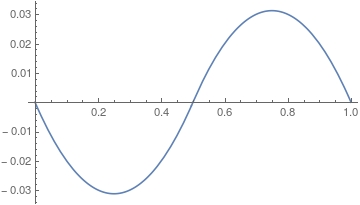
\includegraphics[scale=0.6]{img/puenteflotante.png}
\end{figure}

Que como vemos, floa, asi que algo hay mal :D.

\subsection{Extremos fijos y densidad arbitraria}

El planteamiento es igual al caso más simple, pero ahora la función de densidad, $q(x)$, la consideraremos en $C^\infty$. Sin la expresión de la función $q(x)$, no podemos resolver el problema de forma explícita, pero sí podemos asegurar la existencia de solución. El siguiente procedimiento lo repetiremos varias veces: definimos un espacio en donde buscaremos nuestra solución ($\sobolevcero[0,1]{1}$), plantearemos el problema (condición de extremal), definiremos un producto escalar y demostraremos que el espacio definido con ese producto escalar es de Hilbert, para usar el Teorema de Riesz-Fréchet. 

Comencemos definiendo nuestro espacio de soluciones:
\[
\sobolevcero[a,b]{1}=\conjunto{y\in\sobolev{1}: y(a)=y(b)=0}
\]
Recordemos que en este espacio están las funciones de $\lebesgue{2}$, que tienen derivada débil. Por lo tanto, por la proposición \ref{representantecontinuo} podemos elegir una $y$ que sea continua.
\begin{prop}
El espacio vectorial $\sobolevcero{1}$, es cerrado.
\end{prop}   
\begin{proof}
Sea una secuencia de funciones convergentes en $\sobolevcero{1}$, $f_n\longrightarrow f$. Usando la proposición \ref{inclusion continua} y $\sobolevcero{1}\subset\sobolev{1}$, tenemos que $f_n(a)\longrightarrow f(a)$ y $f_n(b)\longrightarrow f(b)$. Luego $f_n(a)=f_n(b)=0 \;\forall n\in\N \Rightarrow f(a)=f(b)=0 \Rightarrow f\in\sobolevcero{1}$.\\
\end{proof}

Una vez definido nuestro nuevo espacio, pasamos a resolver el modelo. Como de costumbre, suponemos que $y\in\sobolevcero[0,1]{1}$ es extremal y usamos la teoría de Euler:
\[
L(y)=\frac{1}{2}\integral{0}{1}{y'(x)^2dx}+\integral{0}{1}{q(x)y(x)dx}
\]
Usando la notación usual:
\[
L(y)=\integral{0}{1}{F(x,y,p)dx} \; \text{ donde } \;\; F(x,y,p)=\frac{1}{2}p^2+q(x)y
\]
Calculando sus derivadas parciales
\[
F_p(x,y,p)=p \espacio F_y(x,y,p)=q(x)
\]
podemos calcular $\funcion{DL_y}{\sobolevcero[0,1]{1}}{\R}$ y usar la concidición de extremal de $y$ (teorema \ref{theorem:1.7}):
\[
DL_y(\phi)=\integral{0}{1}{y'(x)\phi'(x)dx}+\integral{0}{1}{q(x)\phi(x)dx}=0 \espacio \forall \phi\in\sobolevcero[0,1]{1}
\]
Si lo miramos como una derivada débil, vemos que si $Z(x)=y'(x) \Rightarrow Z'(x)=q(x) \Rightarrow y''(x)=q(x)$, en sentido débil.
\begin{definition}
\label{soluciondebil}
$y\in\sobolevcero{1}$ es \textit{solución débil} de $y''(x)=q(x) \; \forall x 
\in [a,b]$, si se verifica:
\[
\integral{0}{1}{y'(x)\phi'(x)dx}+\integral{0}{1}{q(x)\phi(x)dx}=0 \espacio \forall \phi\in\sobolevcero[0,1]{1}
\]
\end{definition}
Cabe resaltar, el hecho de que en la anterior definición, $y$ está en $\sobolevcero[0,1]{1}$ y estamos resolviendo una EDO de segundo orden, es decir, no sabemos nada sobre la segunda derivada de $y$ (solo de la primera).

Definimos un producto escalar en $\sobolevcero[a,b]{1}$ y veamos que es de Hilbert:
\begin{prop}
El espacio $\sobolevcero[a,b]{1}$ con el siguiente producto escalar:
\[
f,g\in\sobolevcero[a,b]{1}, \espacio <f,g>=\integral{a}{b}{f'(x)g'(x)dx}
\]
es un espacio de Hilbert.
\end{prop}
\begin{proof}
Sea $f_n\in\sobolevcero{1} \;\forall n\in\N$ una sucesión de Cauchy, entonces:
\[
\forall \varepsilon>0 \; \exists n_0: \; n,m\geq n_0 \; \norm{f_n-f_m}_{\sobolevcero{1}}<\varepsilon
\]
Recordemos que si tenemos un producto escalar definido, podemos expresar la norma de un elemento del espaico como la raíz cuadrada del producto escalar de el elemento consigo mismo, es decir:
\[
\norm{f}_{\sobolevcero{1}}=\sqrt{<f,f>}
\]
Usando esa propiedad:
\[
\varepsilon > \norm{f_n-f_m}_{\sobolevcero{1}}=\sqrt{<f_n-f_m,f_n-f_m>}=\sqrt{\integral{a}{b}{(f_n(x)-f_m(x))^2dx}}=\norm{f_n'-f_m'}_2
\]
Luego $f_n'$ converge a una cierta $g$ en $\lebesgue{2}$. Definiendo:
\[
\tilde{f_n}(x)=\integral{a}{b}{f_n'(s)ds} \Rightarrow \tilde{f_n}(x) \longrightarrow \integral{a}{x}{g(s)ds} \Rightarrow f(x) = \limitemasinfinito{n}{\tilde{f_n}(x)}
\]
Ya tenemos nuestro candidato a límite, comprobemos que pertenece a $\sobolevcero{1}$:
\begin{itemize}
\item $f(a)=0$ y $f(b)=\integral{a}{b}{g(s)ds}=f_n'(b)-f_n'(a)=0$.
\item $f$ tiene derivada débil (igual a $g$) por el teorema \ref{fundamentalcalculo}.
\end{itemize}
Luego $f\in\sobolevcero{1}$.
Por último, vemos que converge:
\[
\norm{f_n-f}_{\sobolevcero{1}}=\norm{f_n'-g}_2\longrightarrow 0
\]
\end{proof}

Una vez comprobado que el espacio es de Hilbert, solo nos falta recordar el Teorema de Riesz-Fréchet:
\begin{theorem}[Riesz-Fréchet]
\label{riesz-frechet}
Si $H$ es un espacio de Hilbert y $f\in H^*$, existe $y\in H$ tal que:
\[
f(x)=<x,y> \; \forall x\in H
\]
\end{theorem}

Sea ahora $\phi\in\sobolevcero{1}$, definimos $\funcion{R}{\sobolevcero{1}}{\R}$ por $R(\phi)=-\integral{a}{b}{q(x)\phi(x)dx}\in\left(\sobolevcero{1}\right)^*$. Por el teorema de Riesz-Fréchet, existe $y\in\sobolevcero{1}$ tal que $R(\phi)=<y,\phi>$.

Si desarrollamos la última expresión, nos damos cuenta de que es igual a la condición en la definición \ref{soluciondebil}, que es justo lo que buscábamos.
%\chapter{Teorema de Lax-Milgran}

Para dejar el puente libre, primero necesitamos ver nuestro funcional $L$ desde otro punto de vista. Para ello, vamos a ver una serie de definiciones y propiedades abstractas sobre los \textit{funcionales cuadráticos}, lo que nos va a permitir enunciar el teorema de Lax-Milgran, que nos dará la existencia de solución en esta última versión del modelo.

\begin{definition}\label{formabilineal}
Dados un cuerpo $K$ y un $K-$espacio vectorial $V$, una forma bilineal es una aplicación $\funcion{f}{V\times V}{K}$ que verifica:
\begin{enumerate}[(a)]
\item $f(u_1+u_2,v)=f(u_1,v)+f(u_2,v)$
\item $f(u, v_1+v_2)=f(u,v_1)+f(u,v_2)$
\item $f(au,v)=af(u,v)$
\item $f(u,av)=af(u,v)$
\end{enumerate}
para cualquier $a\in K$ y $u,v,u_1,u_2,v_1,v_2\in V$.

Una propiedad que necesitaremos es:
\[
f\left(\sum_ia_iu_i,\sum_jb_jv_h\right)=\sum_i\sum_ja_ib_jf(u_i,v_j)
\]

\end{definition}

\begin{definition}
Una forma bilineal $\funcion{f}{V\times V}{K}$ se dice simétrice si verifica:
\[
f(u,v)=f(v,u) \espacio \forall u,v\in V
\]
\end{definition}

\begin{definition}
Sea $H$ un espacio de Hilbert arbitrario, $\funcion{A}{H\times H}{\R}$ una forma bilineal, continua y simétrica y $\funcion{R}{H}{\R}$ una aplicación lineal y continua. Llamamos funcional cuadrático a la aplicación $\funcion{L}{H}{\R}$ dada por
\[
L(y)=\frac{1}{2}A(y,y)-R(y) \espacio\forall y\in H
\]
\end{definition}

\begin{definition}
Sea $\funcion{L}{H}{\R}$ una forma cuadrática. Diremos que es coerciva si existe una constante $\alpha\in\R^+$ tal que:
\[
A(u,u)\geq \alpha\norm{u}^2 \espacio \forall u\in H
\]
\end{definition}

\begin{prop}
Sea un espacio de Hilbert $H$ y $\funcion{L}{H}{\R}$ una forma cuadrátrica en ese espacio.
Entonces, la aplicación $\funcion{\norm{\cdot}_H}{H}{\R^+_0}$ definida por 
\[
\norm{u}_H=\sqrt{A(u,u)} \espacio \forall u\in H
\]
donde $\funcion{A}{H\times H}{\R}$ es la forma bilineal asociada a $L$, es una norma, y es equivalente a la norma natural de $H$.
\end{prop}
\begin{proof}
El hecho de que $\norm{\cdot}_H$ es una norma es sencillo de comprobar ya que $A$ define un producto escalar en $H$.

Sea $\funcion{\norm{\cdot}}{H}{\R}$ la norma de $H$. Necesitamos encontrar dos constante $c_1,c_2\in\R^+$ tal que 
\[
c_1\norm{u}\leq \norm{u}_H \leq c_2\norm{u}
\]
La constante $c_2$ la obtenemos por continuidad de la norma $\norm{\cdot}_H$ y la constante $c_1$ de la coercividad de $L$.

\end{proof}
A partir de ahora consideramos $\norm{\cdot}_H$ como nuestra norma por defecto en $H$.
\begin{prop}
Todo funcional cuadrático coercivo está acotado inferiormente.
\end{prop}
\begin{proof}
Sea $\funcion{L}{H}{\R}$ un funcional cuadrático, donde $\funcion{A}{H\times H}{\R}$ es su forma bilineal, continua y simétrica y $\funcion{R}{H}{\R}$ es su aplicación lineal y continua.
Vamos a ver que podemos acotar inferiormente la expresión de $L(y)$, con $y\in H$, por una función parabólica hacia arriba.

Como $R$ es continua, entonces $\norm{R(y)}\leq \norm{R}\norm{y} \Rightarrow -\norm{R(y)} \geq -\norm{R}\norm{y}$. Además, como $L$ es coerciva, existe cierta constante $C\in\R^+$ tal que $A(y,y)\geq C\norm{y}^2$. Combinando esas dos acotaciones, obtenemos:
\[
L(y)=\frac{1}{2}A(y,y)-R(y)\geq \frac{1}{2}C\norm{y}^2-\norm{R}\norm{y}
\]
Para ver con más claridad la parábola, hacemos el cambio $s=\norm{y}$, obteniendo una nueva función $P$ dependiente de las dos constantes $C$ y $\norm{R}$: $P(s)=\frac{1}{2}s^2-s\norm{R}$. Derivando e igualando a 0, obtenemos fácilmente que el mínimo de la parábola $P$ se alcanza en $s=\frac{\norm{R}}{C}$. Luego:
\[
L(y)\geq \frac{\norm{R}}{C} \espacio \forall y\in H 
\]

\end{proof}

\begin{theorem}[Lax-Milgran]
\label{laxmilgran}
Sea $\funcion{L}{H}{\R}$ un funcional cuadrático. Si $L$ es coercivo, entonces tiene mínimo absoluto en $H$.
\end{theorem}

\begin{prop}[condición de punto crítico]
\label{puntocritico}
Sea $\funcion{L}{H}{\R}$ un funcional cuadrático coercivo, $y\in H$, $\phi\in\soportecompacto$. Entonces existe $y\in H$ verificando:
\[
A(\phi,y)-R(\phi)=0 \espacio \forall\phi\in\soportecompacto
\]

Además, el punto $y$ es el mínimo de $L$.
\end{prop}
\begin{proof}
Calculemos primero la expresión explícita de $g(s)$:
\[
g(s)=L(y+s\phi)=\frac{1}{2}A(y+s\phi,y+s\phi)-R(y+s\phi)
\]
Desarrollamos el primer término (usando la última propiedad en la definición \ref{formabilineal}):
\[
A(y+s\phi,y+s\phi)=A(y,y)+sA(y,\phi)+sA(\phi,y)+s^2A(\phi,\phi)=s^2A(\phi,\phi)+2sA(\phi,\phi)+A(y,y)
\]
Para el segundo término, usamos que $R$ es lineal:
\[
R(y+s\phi)=R(y)+sR(\phi)
\]
Quedándo:
\[
g(s)=\frac{1}{2}\left(s^2A(\phi,y)+2sA(\phi,\phi)+A(y,y)\right)-R(y)-sR(\phi)
\]
Derivando respecto de $s$:
\[
g(s)=sA(\phi,\phi)+A(\phi,y)-R(\phi) \Rightarrow g'(0)=A(\phi,y)-R(\phi)
\]
Luego nuestra condición de punto crítico es:
\[
A(\phi,y)-R(\phi)=0 \espacio \forall\phi\in\soportecompacto
\]

Para le existencia, simplemente tenemos que definir un producto escalar y usar el teorema de Riesz, como en los ejemplos anteriores. Sea $<<u,v>>=A(u,v)$ un producto escalar en $H$, por el teorema \ref{riesz-frechet}, existe $y\in H$ verificando:
\[
<<y,\phi>>=R(\phi) \espacio \forall \phi\in\soportecompacto
\]

Para ver que es mínimo, tomamos $\funcion{g}{\R}{\R}$ definida por $g(s)=L(y+s(z-y))$. Notemos que $y+s(z-y)$ es la recta que una a $z$ con $y$. Tenemos que ver
\[
L(z)>L(y) \espacio \forall z\in H
\]
Que si nos fijamos, es equivalente a ver que
\[
g(1)>g(0)
\]
Que ya lo tenemos porque $s=0$ era el punto mínimo de la parábola.
\end{proof}

Una vez planteada toda la teoría necesaria, podemos volver a nuestro modelo del puente. Recordemos que nuestro funcional  $\funcion{L}{\sobolev{1}}{\R}$ venía dado por la expresión:
\[
L(y)=\frac{1}{2}\integral{a}{b}{y'(x)^2dx}+\frac{1}{2}\integral{a}{b}{K(x)y(x)^2dx}+\integral{a}{b}{q(x)y(x)dx}
\]
donde $q,K\in\lebesgue{\infty}$ y $K(x)\geq k_0 >0\ \casipordoquier$. La última condición la imponemos porque al dejar los extremos sueltos (lo hemos hecho al considerar como dominio de $L$ el espacio $\sobolev{1}$ en lugar de $\sobolevcero{1}$) necesitemos que el puente siga enganchado por las cuerdas.

Para poder usar la teoría desarrollada anteriormente, necesitamos ver que nuestro funcional es cuadrático. Definimos nuestra forma bilineal, continua y simétrica, y nuestra aplicación lineal y continua:
\[
A(u,v)=\integral{a}{b}{u'(x)v'(x)dx}+\integral{a}{b}{K(x)u(x)v(x)dx}, \; \espacio R(u)=-\integral{a}{b}{q(x)u(x)dx} \;\;\forall u,v\in\sobolev{1}
\]
Pero también necesitamos que $L$ sea coerciva. Usando la hipótesis sobre $K(x)$ es fácil de ver:
\[
A(u,u)=\integral{a}{b}{u'(x)^2dx}+\integral{a}{b}{K(x)u(x)^2dx}\geq\normasobolev{1}{u}^2+k_0\normasobolev{1}{u}^2\geq(1+k_0)\normasobolev{1}{u}^2
\]
Por lo tanto, sabemos que existe mínimo en $\sobolev{1}$. Además de saber que existe, queremos saber algo más sobre su expresión. Como hemos visto antes, los puntos críticos están caracterizados por la expresión:
\[
y\in\sobolev{1} \text{ punto critico } \Leftrightarrow A(y,\phi)=R(\phi) \espacio \forall \phi\in\sobolev{1}
\]
es decir,
\[
\integral{a}{b}{y'(x)\phi'(x)dx}+\integral{a}{b}{K(x)y(x)\phi(x)dx}=-\integral{a}{b}{q(x)\phi(x)dx} \espacio  \forall\phi\in\sobolev{1}
\]
Si en lugar de considerar $\phi$ en $\sobolev{1}$, la consideramos en $\soportecompacto$. Vemos que llamando $z=y'$ y agrupando los términos que tienen $\phi$, llegamos a:
\[
\integral{a}{b}{z(x)\phi'(x)dx}=-\integral{a}{b}{(K(x)y(x)+q(x))\phi(x)dx} \espacio  \forall\phi\in\sobolev{1}
\]

lo que significa que la derivada débil de $z$ es justamente $ky+q$. En particular z está en $\sobolev{1}$, porque todas las funciones que aparecen están en $\lebesgue{2}$. Luego debemos resolver la siguiente ecuación diferencial de orden 2 en $y$:
\[
y''(x)=K(x)y(x)+q(x) \espacio \forall x \in[a,b]
\]
Si imaginamos que $K$ y $q$ son continuas, esa ecuación tendría un gran número de soluciones. De hecho, el conjunto de soluciones sería un espacio biparamétrico (porque la solución depende de las condiciones iniciales sobre $y$ e $y'$). Tenemos que intentar limitarlas de alguna forma.

\begin{prop}\label{productoh1}
Sea $y\in\sobolev{1}$ (el representante continuo) y $\phi\in\mathcal{D}(\R)$, entonces $y\phi\in\sobolev{1}$.
\end{prop}
\begin{proof}
Para ver que $y\phi\in\sobolev{1}$, necesitamos encontrar su derivada débil. ¿Cuál es nuestro candidato a derivada débil? La derivada clásica, es decir, $z=y'\phi+y\phi'$. Para comprobarlo, tenemos que ver que para toda $\psi\in\soportecompacto$ se tiene:

\[
\integral{a}{b}{(y'(x)\phi(x)+y(x)\phi'(x))\psi(x)dx}+\integral{a}{b}{y(x)\phi(x)\psi'(x)dx}=0
\]
Reordenando los términos que tienen $y$ e $y'$, obtenemos:
\[
\integral{a}{b}{[\phi(x)\psi'(x)+\phi'(x)\psi(x)]y(x)dx}+\integral{a}{b}{[\phi(x)\psi(x)]y'(x)dx}=0
\]
Se cumple que si
$\phi \in \mathcal{D}(\mathbb{R}), \psi \in \mathcal{D}((a,b))$
entonce $\phi\psi \in \mathcal{D}((a,b))$ y
\[
  (\phi\psi)' = \phi'\psi + \phi\psi'
\]
Ahora por ser $y \in \mathcal{H}^1(a,b)$ y
$\hat\phi \in \mathcal{\mathbb{R}}$ tenemos que se cumple
\[
\integral{a}{b}{y'(x)\hat\phi(x)}+\integral{a}{b}{y(x)\hat\phi'(x)}=y(x)\hat\phi(x)\Big|^b_a
\]
una expresión general. Tomando $\hat\phi = \phi\psi$ tenemos que 

\[
\integral{a}{b}{y'(x)\hat\phi(x)}+\integral{a}{b}{y(x)\hat\phi'(x)}=y(x)\hat\phi(x)\Big|^b_a = 0
\]
ya que $\phi\psi(b) = \phi\psi(a) = 0$ y obtenemos así el resultado que buscabamos.
\end{proof}

Volviendo al problema original teníamos que

\begin{equation}
  \label{eq:probleminicial}
  \integral{a}{b}{y'(x)\phi(x)}+\integral{a}{b}{k(x)y(x)\phi(x)}=-\integral{a}{b}{q(x)\phi(x)}
\end{equation}


Considerando $\phi \in \mathcal{D}(\mathbb{R}), \phi \in \mathcal{H}^1$ y $z = y'$

obtenemos en la expresión anterior

\begin{equation}
  \label{eq:resparcial}
  \integral{a}{b}{z\phi'}=z\phi(x)\Big|^b_a - \integral{a}{b}{z'\phi}
\end{equation}

Como estabamos resolviendo el problema $y''=ky + q$ tenemos que se cumple

\[
\integral{a}{b}{z'\phi} = \integral{a}{b}{k(x)y(x)+q(x)\phi}
\]

y usando la igualdad que nos da \ref{eq:probleminicial} despejamos en
\ref{eq:resparcial} y obtenemos
\[
y'\phi\Big|^b_a = 0
\]

Si tomamos una $\phi$ como la siguiente

\centerline{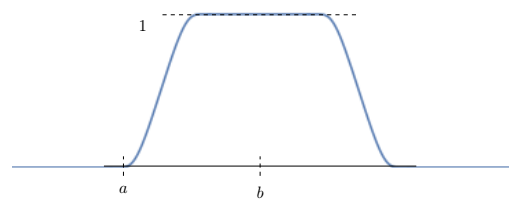
\includegraphics[scale=0.5]{img/caso1.png}} 

de la expresión $ 0 = y'\phi\Big|^b_a = y'(b)\phi(b)-y'(a)\phi(a)$
obtenemos $y'(b) = 0$. Tomando como $\phi$

\centerline{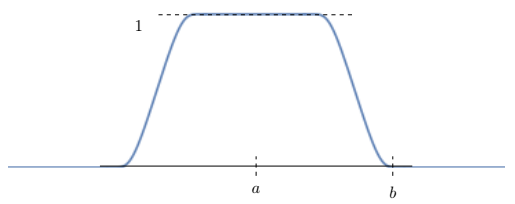
\includegraphics[scale=0.5]{img/caso2.png}} 

obtenemos $y'(a) = 0$. Dado que $z=y'\in \mathcal{H}^1$ entonces $y\in \mathcal{H}^2$ y
tomando el representante continuo obtenemos lo que se conoce como la condición de Neumann.

\section{La delta de Dirac y el espacio $H^{-1}$}

Ahora vamos a ver otro caso del modelo, donde colgamos una masa $m$ en un punto $\alpha\in(a,b)$ del puente. La energía de este objeto es $my(\alpha)$, luego la expresión de nuestro funcional $\funcion{L}{\sobolevcero{1}}{\R}$ es:
\[
L(y)=\frac{1}{2}\integral{a}{b}{y'(x)^2dx}+\frac{1}{2}\integral{a}{b}{q(x)y(x)^2dx}+my(\alpha)
\]
donde $y\in\sobolevcero{1}$, $q(x)\geq 0$ y  $q\in\lebesgue{\infty}$. La intuición nos dice que al colgar la masa $m$, se formará un pico en la cuerda, como muestra el siguiente dibujo:

\begin{center}
\begin{tikzpicture}
\draw (0,0) -- (5,0);
% parabola
\draw[scale=1,domain=0:2.5,smooth,variable=\x,red] plot ({\x}, {-0.2*\x});
\draw[scale=1,domain=2.5:5,smooth,variable=\x,red] plot ({\x}, {0.2*(\x-5)});

% etiquetas
\draw[dashed] (0,-0.7) -- (0,.2);
\draw (0,-0.7) node[anchor=north] {$a$};
\draw[dashed] (5,-.7) -- (5,.2);
\draw (5,-0.7) node[anchor=north] {$b$};
\draw (2.5,-0.1) -- (2.5,.1);
\draw (2.5,0) node[anchor=north] {$\alpha$};
\draw (3,-0.7) node[anchor=north] {$m$};

% masa
\fill[blue!40!white, draw=black] (2.25,-1) rectangle (2.75,-0.5);
\end{tikzpicture}
\end{center}
La forma bilineal $A$ es la misma que en el anterior modelo:
\[
A(y,y)=\frac{1}{2}\integral{a}{b}{y'(x)^2dx}+\frac{1}{2}\integral{a}{b}{q(x)y(x)^2dx}
\]
y como estamos en $\sobolevcero{1}$, $\integral{a}{b}{y'(x)^2dx}$ es una norma, luego $A$ es coercivo ya que restando el último término (que es positivo) obtenemos:
\[
A(y,y)\geq \frac{1}{2}\integral{a}{b}{y'(x)^2dx} = \frac{1}{2}\norm{u}^2
\] 
La aplicación lineal y continua $\funcion{R}{\sobolevcero{1}}{\R}$, viene dada por $R(y)=-my(\alpha)$, que tiene sentido al elegir el represante continuo porque $\sobolev{1}\subset \mathcal{C}(a,b)$. Por el teorema de Lax-Milgran (\ref{laxmilgran}) y la proposicion \ref{puntocritico}, existe $y\in\sobolevcero{1}$ de forma que
\[
A(y,\phi)=R(\phi) \espacio \forall \phi\in\sobolevcero{1}
\]
Lo que vamos a hacer ahora es calcular o ver qué condiciones verifica la función $y$. Usando la condición de punto crítico:
\begin{equation}
\label{formulageneral}
\integral{a}{b}{y'(x)\phi'(x)dx}+\integral{a}{b}{q(x)y(x)\phi(x)dx}=-m\phi(\alpha)
\end{equation}
Ahora hacemos una distinción de casos con $\phi$ perteneciendo a diferentes clases de Swartz:
\begin{itemize}[-]
\item si $\phi\in\mathcal{D}(a,\alpha)$:
\[
\integral{a}{b}{y'(x)\phi'(x)dx}+\integral{a}{b}{q(x)y(x)\phi(x)dx}=-m\phi(\alpha)=0
\]
ya que $\alpha\notin(a,\alpha) \Rightarrow \phi(\alpha)=0$. Si denotamos $z=y'$, entonces $z\in\sobolev[a,\alpha]{1}\subset\mathcal{C}[a,\alpha]$ (porque la expresión anterior coincide con la definición de derivada débil para $z$).
\item si $\phi\in\mathcal{D}(\alpha,b)$, de igual forma conseguimos que $z\in\sobolevcero[\alpha,b]{1}\subset\mathcal{C}[\alpha,b]$. 
\end{itemize}
Fijaros que ese razonamiento no implica que $z\in\mathcal{C}[a,b]$, ya que el representante continuo usado en $[a,\alpha]$ y $[\alpha,b]$ son distintos. Lo que si implica es que $z\in\mathcal{C}\left([a,\alpha]\right)\cap \mathcal{C}\left([\alpha,b]\right)$ y existen los límites laterales de $\alpha$:
\[
z(\alpha^-)=\limite{x}{\alpha^-}{z(x)} \espacio z(\alpha^+)=\limite{x}{\alpha^+}{z(x)}
\]
Además sabemos que $z'=qy \;\; a.e \; x \in(a,\alpha)\cup(\alpha,b)$. Si volvemos a la fórmula general \eqref{formulageneral}:
\begin{equation}
\label{formulageneral2}
\integral{a}{b}{z(x)\phi'(x)dx}+\integral{a}{b}{q(x)y(x)\phi(x)dx}=-m\phi(\alpha) \espacio \forall\phi\in\sobolevcero{1}
\end{equation}
Ahora queremos desarrollar esa expresión. Tomamos $\phi\in\soportecompacto$, como $z$ no es continua en $\alpha$, la integral del primer término hay que escribirla en dos partes:
\[
\integral{a}{b}{z(x)\phi'(x)dx}=\integral{a}{\alpha}{z(x)\phi'(x)dx}+\integral{\alpha}{b}{z(x)\phi'(x)dx}
\]
Aplicamos derivación por partes a cada término:
\[
\integral{a}{\alpha}{z(x)\phi'(x)dx}=z(x)\phi(x)\Big|_a^\alpha-\integral{a}{\alpha}{z'(x)\phi(x)dx}=z(\alpha^-)\phi(\alpha)-\integral{a}{\alpha}{z'(x)\phi(x)dx}
\]
\[
\integral{\alpha}{b}{z(x)\phi'(x)dx}=z(x)\phi(x)\Big|_\alpha^b-\integral{\alpha}{b}{z'(x)\phi(x)dx}=-z(\alpha^+)\phi(\alpha)-\integral{\alpha}{b}{z'(x)\phi(x)dx}
\]
Combinando los resultados y sustituyendo en \eqref{formulageneral2}:
\[
z(\alpha^-)\phi(\alpha)-z(\alpha^+)\phi(\alpha)-\integral{a}{b}{z'(x)\phi(x)dx}=-\integral{a}{b}{z'(x)\phi(x)dx}-m\phi(\alpha)
\]
Cancelando ámbos términos:
\[
\left(z(\alpha^-)-z(\alpha^+)\right)\phi(\alpha)=-m\phi(\alpha)
\]
Como la función de Swartz escogida es arbitraria, podemos suponer que vale 1 en $\alpha$. Usando eso y que $z=y'$:
\[
y'(\alpha^-)-y'(\alpha^+)=-m \Rightarrow y'(\alpha^+)-y'(\alpha^-)=m  
\]
Es decir, el cambio de pendiente que se da entre $\alpha^-$ y $\alpha^+$ es igual a $m$, el peso de la masa.

\section{Sturm-Liouville: caso 1}

Vamos a generalizar el caso anterior para obtener una ecuación diferencial con varias condiciones. Sea $\funcion{L}{\sobolev{1}}{\R}$ el funcional dado por:
\[
L(y)=\frac{1}{2}\integral{a}{b}{y'(x)^2dx}+\frac{1}{2}\integral{a}{b}{q(x)y(x)^2dx}-R(y)
\]
con $q\in\lebesgue{\infty}$, $0<q_0\leq q(x)\leq q_1 \; \casipordoquier$. 

De donde podemos definir la siguiente forma cuadrática: 
\[
A(y,\phi)=\integral{a}{b}{y'(x)\phi'(x)dx}+\integral{a}{b}{q(x)y(x)^2\phi(x)dx}
\]
Una vez más, la teoría de Lax-Milgran nos dice que existe $y$ en $\sobolev{1}$ cumpliendo $A(y,\phi)=R(\phi)$, es decir, $ \forall R\in \sobolev{-1}=\left(\sobolev{1}\right)^*$:
\begin{equation}
\label{condicion1}
\integral{a}{b}{y'(x)\phi'(x)dx}+\integral{a}{b}{q(x)y(x)\phi(x)dx}=R(\phi) \;\; \forall \phi\in\sobolev{1}
\end{equation}

Una vez planteado el problema y visto que tiene solución, tenemos que intentar determinar $y$ mediante alguna ecuación diferencial. Como vamos a determinar $y$ mediante una ecuación diferencial, necesitamos buscar condiciones de regularidad sobre ella porque la teoría de ecuaciones diferenciales nos dice que hay solución siempre que los elementos de la ecuación sean continuos. Nótese que, por ahora, solo sabemos que $y\in\continuas$ e $y'\in\lebesgue{2}$.
   
Ahora vamos a empezar con el primer caso. Partimos de la condición \eqref{condicion1} y recordamos que tenemos la cadena de espacios:
\[
\lebesgue{2} = \sobolev{0} \subset \sobolev{-1}
\]

Donde la indentificación $\sobolev{0}\longhookrightarrow\sobolev{-1}$ viene dada por la aplicación
\[
\begin{array}{ll}
R: & \lebesgue{2} \longrightarrow \sobolev{-1} \\
  &\;\;\; r \;\;\; \;\;\;\; \longmapsto    \funcion{R_r}{\sobolev{2}}{\R} \\
  & \hspace*{3cm} y \mapsto R_r(y)=\integral{a}{b}{r(x)y(x)dx} 
\end{array}
\]

Nótese ahora que si denotamos $z=y'$, la ecuación \eqref{condicion1} nos dice que se verifica:
\begin{equation}
\label{condicion2}
\integral{a}{b}{z(x)\phi'(x)dx}+\integral{a}{b}{q(x)y(x)\phi(x)dx}=\integral{a}{b}{r(x)\phi(x)dx}
\end{equation}
Y agrupando:
\[
\integral{a}{b}{z(x)\phi'(x)dx}+\integral{a}{b}{\left(q(x)y(x)-r(x)\right)\phi(x)dx}=0
\]
Luego $z$ tiene derivada débil y coincide con $z'=qy-r$. Como $z'=y''$, nos queda la EDO:
\[
y''-qy=-r \Rightarrow -y''+qy=r
\]
Ahora, como $z$ tiene derivada débil, puedo tomar su representante continuo $\bar{z}\in\continuas$, es decir, podemos suponer directamente que $z\in\continuas$. Pero claro, como $z=y'$, entonces $y'\in\continuas$, lo que implica que $y\in\continuas[1]$. En particular, tenemos definido cuanto vale $y'(a)$ e $y'(b)$ (antes no lo teníamos porque solo sabíamos que $y\in\lebesgue{2}$). Luego la ecuación $-y''+qy=r$ se verifica en $\sobolev{2}$ (porque $z\in\sobolev{1}$, luego $y\in\sobolev{2}$).

Se puede comprobar fácilmente que si $r,q\in\continuas$ entonces $y\in\continuas[2]$, debido a que en ese caso, $y''$ sería continua (se expresaría como diferencia de continuas y producto de continuas).

Como la expresión \eqref{condicion2} es válida para toda $\phi\in\sobolev{1}$, podemos tomar una $\phi\in\mathcal{D}(\R)$ y como $z\in\sobolev{2}$, la proposición \ref{productoh1} nos dice que $z\phi\in\sobolev{1}$ y $\left(z\phi\right)'=z\phi'+z'\phi$. Usando integración por partes en el primer término:
\[
\integral{a}{b}{z(x)\phi'(x)dx}=z(x)\phi(x)\Big|_a^b-\integral{a}{b}{z'(x)\phi(x)dx}=
\]
\[
=z(b)\phi(b)-z(a)\phi(a)-\integral{a}{b}{(q(x)y(x)-r(x))\phi'(x)dx}
\]
Sustituyendo ahora lo obtenido en la expresión \eqref{condicion2} y simplificando, llegamos a:
\[
z(b)\phi(b)-z(a)\phi(a)=0 \espacio \forall \phi \in\mathcal{D}(\R)
\]
Si ahora tomamos una función $\phi$ de la siguiente forma:

\centerline{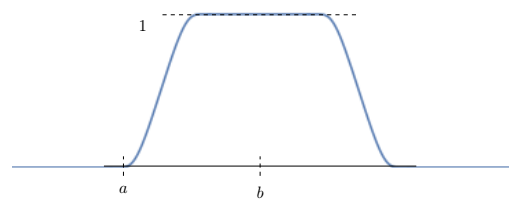
\includegraphics[scale=0.5]{img/caso1.png}} 

Entonces $\phi(a)=0$ y $\phi(b)=1$, de donde queda que $z(b)=0$. Tomando otra $\phi$ de esta forma
\centerline{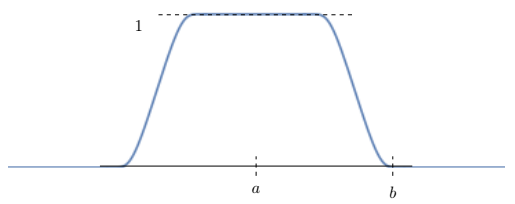
\includegraphics[scale=0.5]{img/caso2.png}} 

obtenemos que $z(a)=0$. Es decir, $y'(a)=y'(b)=0$.

\section{Sturm-Liouville: caso 2}

Para al siguiente caso tenemos que definir primero la \textit{delta de Dirac}.

\medskip

\begin{definition}
Dado $\alpha\in(a,b)$, definimos la función $\funcion{\delta_\alpha}{\sobolev{-1}}{\R}$
\[
\delta_\alpha(y)=y(\alpha), \espacio \delta_\alpha\in\sobolev{1}, \;\; \delta_\alpha\notin\sobolev{0}
\]
A $\delta_\alpha$ se le llama $\delta$ de Dirac.
\end{definition}
\begin{remark}
Nótese que esta función simplemente es otra forma de denotar la evaluación en $\alpha$, que usamos para indicar en qué punto ($\alpha$) de una cuerda ($y$) colgamos una masa $c$. 
\end{remark}

Ahora pasamos al siguiente caso, donde suponemos que $R(\phi)=c\delta_\alpha(\phi)=c\phi(\alpha) \espacio \forall \phi\in\sobolev{1}\subset\continuas$, con $a<\alpha<b$. Con esta nueva $R$, vemos otra vez la ecuación \ref{condicion1} con $z=y'$:
\[
\integral{a}{b}{z(x)\phi'(x)dx}+\integral{a}{b}{q(x)y(x)\phi(x)dx}=c\phi(\alpha)
\]
donde solo sabemos que $z\in\lebesgue{2}$ e $y\in\sobolev{1}$ y $z$ no tiene por qué tener derivada débil ya que la expresión anterior no coincide con la de la definición. 

Si ahora considero el intervalo $(a,\alpha)$ y tomo $\phi\in\mathcal{D}(a,\alpha)$, tenemos que $\phi(\alpha)=0$ y
\[
\integral{a}{b}{z(x)\phi'(x)dx}+\integral{a}{b}{q(x)y(x)dx}=0
\]
Luego $z\in\sobolev[a,\alpha]{1}$, que tiene un representante continuo $z_1\in\mathcal{C}[a,\alpha]$. De forma análoga, obtenemos $z_2\in\mathcal{C}[\alpha,b]$. Si definimos $z'$ como la unión de $z_1'$ y $z_2'$:
\[
z'(x)= \left\{
\begin{array}{cc}
z_1'(x) & x\in(a,\alpha) \\
z_2'(x) & x\in(\alpha,b)
\end{array}
\right.
\]
¿y qué pasa con $z'(\alpha)$? No pasa nada, porque $\{\alpha\}$ tiene medida nula asi que no hace falta definirla en ese punto. Además, $z'\in L^2(a,\alpha)$ y $z'\in L^2(\alpha,b)$, luego $z'\in\lebesgue{2}$ por la misma razón. 

Como $z'$ no es la derivada débil de $z$ en $(a,b)$, solo podemos decir que
\[
\integral{a}{b}{z'(x)\phi(x)dx}+\integral{a}{b}{z(x)\phi'(x)dx}=0 \espacio \forall \phi\in\mathcal{D}(a,\alpha) \text{ y } \forall \phi\in\mathcal{D}(\alpha,b)
\]
Y en ese caso, $z'(x)=-q(x)y(x) \;\; \casipordoquier$. 

Como vemos, este es el origen de la cuestión, tenemos una función $z'$, que sabemos que es una derivada, pero es una derivada \textit{extraña}, ya que es débil en $(a,\alpha)$ y $(\alpha,b)$, coincide en casi todo punto con $-q(x)y(x)$, pero no es una derivada débil en $(a,b)$. 

Por la condición de punto crítico, tenemos que:
\[
\integral{a}{b}{z_1(x)\phi'(x)dx}+\integral{a}{b}{q(x)y(x)\phi(x)dx}=0 \espacio \forall\phi\in\mathcal{H}^1(a,b)
\]
Si $phi(x)=0\quad\forall x\geq\alpha$,
\[
\integral{a}{\alpha}{z_1(x)\phi'(x)dx}+\integral{a}{\alpha}{q(x)y(x)\phi(x)dx}=0
\] 
Si igual que en el caso anterior, consideramos $\phi\in\mathcal{D}(\R)$ y aplicamos integración por partes al primer término:
\[
\integral{a}{\alpha}{z_1(x)\phi'(x)dx}=z_1(x)\phi(x)\Big|_a^\alpha-\integral{a}{\alpha}{q(x)y(x)\phi(x)dx}
\]
Cogiendo la $\phi$ de forma que $\phi(a)=1$ y $phi(x)=0\quad\forall x\geq\alpha$ y sustituyendo en la expresión anterior, obtenemos que:
\[
-z_1(a)\phi(a)=0 \Rightarrow z_1(a)=0
\]

Análogamente se prueba que $z_2(b)=0$.

% A partir de aquí no tiene sentido, supongo que está incompleto
Si ahora usamos eso en la expresión:
\[
\integral{a}{b}{z(x)\phi'(x)dx}+\integral{a}{b}{q(x)y(x)\phi(x)dx}=0
\]
Pero claro, el primer término lo podemos partir en dos integrales diferentes:
\[
\integral{a}{b}{z(x)\phi'(x)dx}=\integral{a}{\alpha}{z(x)\phi'(x)dx}+\integral{\alpha}{b}{z(x)\phi'(x)dx}
\]

\subsection{CLASE 31 MARZO}


\chapter{Ley de acción de masas}

Ahora dejamos los puentes y cambiamos a otro tipo de modelos totalmente diferentes. Vamos a hablar de la ley de acción de masas, pero primero vamos a repasar un poco algunas nociones sobre reacciones químicas. Tenemos una serie de productos $A_1,\cdots, A_n$, $B_1,\cdots, B_n$ y una serie de coeficientes que nos indican la concentración de cada producto: $\alpha_1,\cdots, \alpha_n$, $\beta_1,\cdots, \beta_n$. A estos coeficientes se les llama \textit{coeficientes estequiométricos}. Estos elementos nos dan una reacción química, que expresaremos como:
\[
\alpha_1A_1+\cdots+\alpha_nA_n \longrightarrow \beta_1B_1+\cdots+\beta_nB_n
\]
\begin{example} La reacción química de la quema de hidrógeno:
\[
2H_2+0_2\longrightarrow 2H_20
\]
Otra diferente:
\[
ClH+NaOH \longrightarrow ClNa+H_20
\]
\end{example}

Esto es una cuestión molecular y trabajar con ellas es bastante complicado. Para solventar ese problema, usamos los \textit{moles}. Un \textit{mol} es la cantidad de una sustancia que contiene tantos átomos como su peso atómico. También usaremos la \textit{concentración de un producto}, $[N]$, que es el igual al número de moles que hay del producto. En la reacción anterior obtendríamos dos moles de agua, combinando dos moles de hidrógeno y un mol de oxígeno. Podemos hablar de concentración de \textit{reactivos} y \textit{productos}: $[A] = \{ \text{ número de moles de reactivo } \}$, $[B] = \{ \text{ número de moles de producto } \}$

Por otro lado, está la denominada \textit{velocidad de reacción}, que es la variación de la concentración a lo largo del tiempo. La teoría nos dice que:
\[
\frac{d}{dt}[B]=k[A_1]\cdots[A_n]
\]
\begin{example}
Sean $X,Y$ y $Z$ tre compuestos químicos que se combinan en un producto final $F$ según la reacción:
\[
2X+3Y+5Z\longrightarrow 5F
\]
La velocidad de reacción (moléculas más o menos iguales) se puede suponer proporcional al producto de concentraciones de productos $X,Y,Z$, según un coeficiente $\beta$ (velocidad de reacción). Suponemos que $\beta=0.01$. Si partimos inicalmente de 5 moles de $X$, 7 moles de $Y$ y 10 moles de $Z$, plantear un modelo que permita calcular la concentración de cada sustancia en cada instante. ¿Qué pasará tras mucho tiempo?

Básicamente hay que aplicar una regla de 3:
\[
\left.
\begin{array}{ccc}
2X & \longrightarrow & 5F\\
5X & \longrightarrow & ?
\end{array}
\right\} \Rightarrow \text{ se producirían  12.5F}
\]
\[
\left.
\begin{array}{ccc}
3Y & \longrightarrow & 5F\\
7Y & \longrightarrow & ? = 
\end{array}
\right\} \Rightarrow \text{ se producirían  11.6F }
\]
\[
\left.
\begin{array}{ccc}
5Z & \longrightarrow & 5F\\
10Z & \longrightarrow & ? = 10 
\end{array}
\right\} \Rightarrow \text{ se producirían  10F }
\]
De aquí, deduzco que se van a producir 10 moles de $F$, ya que es el mínimo de las 3 reglas que hemos hecho. Ahora tenemos que ver cuanta cantidad queda de los reactivas $X$ e $Y$ al crear 10 moles de $F$.
\[
\left.
\begin{array}{ccc}
2X & \longrightarrow & 5F\\
? & \longrightarrow & 10F
\end{array} 
\right\}
\Rightarrow \text{ se gastan 4X }
\]
\[
\left.
\begin{array}{ccc}
3Y & \longrightarrow & 5F\\
? & \longrightarrow & 10F
\end{array}
\right\} \Rightarrow \text{ se gastan 6Y }
\]
Luego sobran 1 de $X$, 1 de $Y$ y 0 de $Z$, y se habrán creado 10 moles de $F$. Ahora vamos a denotar por $x(t),y(t),z(t),F(t)$ a la concentración de $X,Y,Z,F$ en el instante $t$ respectivamente. En el instante $t=0$, tendremos las concentraciones iniciales, y en el instante $t=1$, tendremos las finales (el resultado de las cuentas que hemos hecho antes), es decir:
\[
\begin{array}{|c|c|c|}
\hline
& t=0 & t=1 \\
\hline
x(t) & 4 & 1\\
\hline
y(t) & 7 & 1\\
\hline
z(t) & 10 & 1\\
\hline
F(t) & 0 & 1\\
\hline
\end{array}
\]
Si nos fijamos, $5-x(t),7-y(t),10-z(t)$ son los restantes de los productos $X,Y,Z$ en el instante $t$. Es decir, tenemos que la velocidad de reacción de $F$ es:
\[
F'(t)=\beta x(t)y(t)z(t)
\]
Haciendo otra regla de 3:
\[
\left.
\begin{array}{ccc}
2X & \longrightarrow & 5F\\
5-x(t) & \longrightarrow & F(t)
\end{array}
\right\} \Rightarrow F(t)=\frac{5(5-x(t))}{2} \Rightarrow x(t)=5-\frac{2F(t)}{5}
\]
De forma análoga, obtenemos las expresiones de $y(t)$ y $z(t)$:
\[
y(t)=7-\frac{3F(t)}{5}, \espacio z(t)=10-F(t)
\]
Es decir, la expresión final de la velocidad de reacción sería:
\[
F'(t)=0.01\left(5-\frac{2F(t)}{5}\right)\left(7-\frac{3F(t)}{5}\right)\left(10-F(t)\right), \espacio F(0)=0
\]

Si llamamos $g(F)=0.01\left(5-\frac{2F}{5}\right)\left(7-\frac{3F}{5}\right)\left(10-F\right)$, que tiene raíces $F=10,35/3,12.5$. 

\begin{center}
\begin{tikzpicture}[scale=0.5]
\draw (0,0) -- (16,0);
% parabola
\draw[scale=1,domain=0:16,smooth,variable=\x,red] plot ({\x}, {0.01*(5-2*\x/5)*(7-3*\x)*(10-\x)});

% etiquetas
\draw[dashed] (2.3,-0.7) -- (2.3,.2);
\draw (2.3,-1) node[anchor=north] {$10$};
\draw[dashed] (10,-0.7) -- (10,.2);
\draw (10,-1) node[anchor=north] {$\frac{35}{3}$};
\draw[dashed] (12.7,-0.7) -- (12.7,.2);
\draw (12.7,-1) node[anchor=north] {$12.5$};

\draw (2,2) node[] {$g(F)$};

\end{tikzpicture}
\end{center}

Ahora vamos a abstraer un poco el problema para no tener que trabajar con todos los números particulares. Supongamos que tenemos el problema de valores iniciales:
\[
\left\{
\begin{array}{l}
x'=g(x) \\
x(0)=x_0, \espacio x_0<\alpha_1
\end{array}
\right.
\]
donde $\funcion{g}{\R}{\R}$, $g(\alpha_1)=0$, $g'(\alpha_1)<0$ (para que sea compatible con el dibujo) (\textbf{duda}), $g(x)>0$ si $x\in(-\infty, \alpha_1)$ y $\alpha_1$ es la primera raíz de $g$. 

Como sabemos, el anterior problema de valores iniciales tiene una solución maximal $\funcion{x}{(w_-,w_+)}{\R}$, que además es única. Probemos ahora, una serie de propiedades.
\begin{itemize}
\item $x(t)<\alpha_1, \text{ si } t\in(w_-,w_+)$

Tomamos $t^*\in(w_-,w_+)$ con $x(t^*)=\alpha_1$, entonces $x$ sería solución del problema de valores iniciales:
\[
\left\{
\begin{array}{l}
x'=g(x) \\
x(t^*)=\alpha_1
\end{array}
\right.
\]
cuya solución es la constante, $x(t)=\alpha_1$ $\forall t\in(w_-,w_+)$. (\textbf{duda: no entiendo esta demostracion x'd})

\item $x'(t)>0$ $\forall t\in(w_-,w_+)$

Usando el punto anterior es fácil, ya que $x'(t)=g(x(t))>0$ porque $g(x)$ es positivo para todo $x$ en $(-\infty, \alpha_1)$

\item Necesariamente se tiene que $w_+=+\infty$.

Si $t\in[0,w_+)$, entonces $x_0\leq x(t) < \alpha_2$. Ahora podemos usar la teoría de prolongación de soluciones, que nos dice que si tenemos una solución acotada, podemos prolongarla. $x$ además de estar acotada, está lejos del borde. 

\item $\limitemasinfinito{t}{x(t)}=\alpha_1$

Como $x(t)$ es creciente y acotada, entonces el límite existe, y valdrá $L\in\R$. Evidentemente, $L\leq \alpha_1$. Lo único que tenemos que ver es que $L=\alpha_1$. Para ello, vamos a recordar un resultado general:
\begin{lemma}
Sea $\funcion{x}{(w_-,+\infty)}{\R}\in\mathcal{C}^1$ con $\limitemasinfinito{t}{x(t)}=L\in\R$. Entonces existe una sucesión $t_n\in(w_-,+\infty)$ tal que $t_n\longrightarrow +\infty$, con $x'(t_n)\longrightarrow m0$.
\end{lemma}
\begin{proof}
Considerando la diferencia $x(n+1)-x(n)$ y aplicando el teorema del valor medio, nos queda que:
\[
x(n+1)-x(n)=x'(t_n)(n+1-n)=x'(t_n)
\]
Como $x(n+1)\longrightarrow L \leftarrow x(n)$, $x'(t_n)\longrightarrow 0$.
\end{proof}
Luego al existir el límite anterior, existe también $t_n\longrightarrow +\infty$ tal que $x'(t_n)\longrightarrow 0$, es decir, $g(x(t_n))\longrightarrow 0$.  Pero $g(x(t_n))\longrightarrow g(L)$, luego $L=\alpha_1$, que es la raíz.
\end{itemize}

Como $\alpha_1$ era la primera raíz de $g$, es decir, $\alpha_1=10$, hemos visto que $F(t)\longrightarrow 10$. Pero ojo, simplemente tiende, nunca llegamos a crear los 10 moles enteros, es una asíntota que no se alcanza en tiempo finito. Además $F(t)<10$ $\forall t \in(0,+\infty)$.

Usando la cota sobre $F(t)$ y recordando la expresión de $x(t)$, llegamos a que:
\[
x(t)=5-\frac{2F(t)}{5}>5-4=1 \Rightarrow x(t)\longrightarrow 1
\]
Igual con la $y(t)$ y $z(t)$:
\[
y(t)=7-\frac{3F(t)}{5}>7-6=1 \Rightarrow y(t)\longrightarrow 1
\]
\[
z(t)=10-F(t) \Rightarrow z(t)\longrightarrow 0
\]

Volvemos otra vez a la parte abstracta. Sea $g\in\mathcal{C}^2$ de la forma:

\begin{center}
\begin{tikzpicture}
\draw (0,0) -- (5,0);
% parabola
\draw[scale=1,domain=0:5,smooth,variable=\x,red] plot ({\x}, {-0.08*\x*\x+1});

% etiquetas
\draw[dashed] (0,-0.7) -- (0,.2);
\draw (0,-0.75) node[anchor=north] {$x_0$};
\draw[dashed] (3.6,-0.7) -- (3.6,.2);
\draw (3.6,-0.75) node[anchor=north] {$x$};
\end{tikzpicture}
\end{center}

cumpliendo $g'(\alpha)=\delta<0$. Entonces vamos a tener que (lo que he visto antes):
\[
\limitemasinfinito{t}{x(t)}=\alpha
\]
Ahora vamos a decir un poquito más. Vamos a probar que:
\[
\limitemasinfinito{t}{\frac{x(t)-\alpha}{e^{\delta t}}}=-L\in(-\infty,0)
\]
Eso quiere decir que la convergencia al valor $\alpha$ es exponencial, es decir, los residuos ($x(t),y(t),z(t)$no sólo tienden a 10, sino que además lo hacen exponencialmente.
\begin{proof}
Calculemos el siguiente límite:
\[
\limitemasinfinito{t}{\frac{x'(t)}{x(t)-\alpha}}=\limitemasinfinito{g(x(t))}{x(t)-\alpha}=\limite{x}{\alpha}{\frac{g(x)}{x-\alpha}}=\delta
\]
Eso nos dice que si tenemos $\beta(t)=\frac{x'(t)}{x(t)-\alpha}$, entonces $\beta(t)\longrightarrow \delta$. Por supuesto, $\beta$ es continua y se verifica la ecuación diferencial:
\[
x'(t)= \beta(t)(x(t)-\alpha)
\]
Usando que $x(t)=\alpha$ es una solución particular de esa ecuación y $x(t)=ce^{-\int_0^t\beta(t)dt}$ es una solución de la homogénea, podemos escribir la solución general:
\[
x(t)=\alpha-ce^{-\int_0^t\beta(t)dt}
\]
donde hemos añadido la solución de la homogénea directamente restando porque sabemos que se tiene que cumplir $x(t)<\alpha$. Diviendo todo por $e^{\delta t}$:
\[
\frac{x(t)-\alpha}{e^{\delta t}}=\frac{-ce^{-\int_0^t\beta(t)dt}}{e^{\delta t}}=-ce^{-\int_0^t\beta(t)dt-\delta t}=-ce^{-\int_0^t\left(\beta(s)-\delta \right)ds}
\]
Ahora ya lo único que queda por ver es que $\beta(s)-\delta$ sea integrable en $(0,+\infty)$. Para eso:
\[
\beta(t)-\delta=\frac{x'(t)}{x(t)-\alpha}-\delta=\frac{g(x(t))-\delta(x(t)-\alpha)}{x(t)-\alpha}=\frac{g(x)-g(\alpha)-g'(\alpha)(x-\alpha) }{x-\alpha}\leq O(x-\alpha)
\]
donde para la acotación por algo de orden $x-\alpha$ hemos usado que $g\in\mathcal{C}^2$, luego:
\[
\beta(t)-\delta\leq O(x(t)-\alpha)
\]
¿Y por qué $x(t)$ es integrable? Debido a que:
\[
x(t)-\alpha = \frac{x(t)-\alpha}{g(x(t))}g(x(t))
\]
y ambos términos están acotados (ya que $g(x(t))=x'(t)$ y $x'(t)$ es integrable).
\end{proof}

Este es el único modelo que vamos a desarrollar con este nivel de detalle, los siguientes serán más escuetos.
\end{example}
%\documentclass[12pt]{article}
 
\usepackage[margin=1in]{geometry} 
\usepackage{amsmath,amsthm,amssymb}
\usepackage[spanish]{babel}
\usepackage[utf8]{inputenc}
\usepackage{tikz-cd}
\usepackage{amsmath}
\usepackage[shortlabels]{enumitem}
\usepackage{mathtools}

% cosas entre comillas 
\usepackage{csquotes}

\usepackage{tikz}


\usepackage{xcolor}

%\usepackage{config}

\newtheorem{theorem}{Teorema}[section]
\newtheorem{lemma}[theorem]{Lema}
\newtheorem{prop}[theorem]{Proposición}
\newtheorem{coro}[theorem]{Corolario}
\newtheorem{conj}[theorem]{Conjetura}
\newtheorem{ejercicio}{Ejercicio}[section]
\newtheorem*{ejercicio*}{Ejercicio}
\theoremstyle{definition}
\newtheorem{definition}[theorem]{Definición}
\newtheorem{example}[theorem]{Ejemplo}
\theoremstyle{remark}
\newtheorem{remark}[theorem]{Nota}
\newtheorem{notacion}[theorem]{Notación}
\newcommand{\continuas}[1][]{C^{ #1 }[a,b]}
\newcommand{\continuasabierto}[1][]{C^{ #1 }(a,b)}
\newcommand{\soportecompacto}{\mathcal{D}(a,b)}
\newcommand{\xcero}{(a,b)}
\newcommand{\xcerocerrado}{[a,b]}
\newcommand{\fvariaciones}{F(x,y(x),y'(x))}

\begin{document}

\section{Ejercicios tema 1}

\begin{ejercicio}
  Sean $\Phi\in \mathcal{C}^1(\mathbb{R}^3), y(x)\in \mathcal{C}^2\xcero, y'(x) \neq 0$. Dado el funcional

  \[
    F[y] = \int_{a}^{b}{\Phi(x,y(x),y'(x))dx}
  \]

  demuéstrese la equivalencia de las dos formas siguientes de las
  ecuaciones de Euler-Lagrange.

  \begin{itemize}
  \item $\frac{\partial\Phi}{\partial y}-\frac{d}{dx}\frac{\partial\Phi}{\partial p} = 0 $
  \item $\frac{\partial\Phi}{\partial x} - \frac{d}{dx}(\Phi-y'\frac{\partial\Phi}{\partial p}) = 0$
  \end{itemize}

  \begin{proof}
    Comenzamos viendo el caso $a) \implies b)$. Para ello en primer
    lugar tenemos que comprobar que efectivamente podemos derivar
    $\Phi$ respecto al tercer parámetro. Del apartado $a)$ sabemos que

    \[
      \frac{\partial\Phi}{\partial y} = \frac{d}{dx}\frac{\partial\Phi}{\partial p}
    \]
    
    y del enunciado sabemos que $\Phi$ es de calse $\mathcal{C}^1$
    luego $\frac{\partial\Phi}{\partial p}$ es de $\mathcal{C}^1$.

    Cuando derivamos $\Phi(x,y(x),y'(x))$ obtenemos

    \begin{align*}
      \Phi(x,y(x),y'(x))' & = \frac{\partial\Phi}{\partial x}(x, y(x), y'(x)) \\
                          & = \frac{\partial\Phi}{\partial y}(x, y(x), y'(x))y'(x) \\
                          & = \frac{\partial\Phi}{\partial p}(x, y(x), y'(x))y''(x)
    \end{align*}

    Recordemos que $\frac{\partial\Phi}{\partial p}(x, y(x), y'(x)) = z(x)$ luego

    \begin{align*}
      \frac{d}{dx}(\Phi-y'\frac{\partial\Phi}{\partial p}) & = \Phi_x + \Phi_yy' + \Phi_py'' - y''z -y'z'
    \end{align*}

    Tenemos que el 3º y 4º termino son iguales t el 2º y 4º son
    iguales entre ellos luego obtenemos

        \begin{align*}
      \frac{d}{dx}(\Phi-y'\frac{\partial\Phi}{\partial p}) = \Phi_x
        \end{align*}

        que es lo que queríamos.

        $b)\implies a)$
        
        Todos los pasos que hemos dado son reversibles pero
        necesitamos ver que
        $\frac{\partial\Phi}{\partial p}(x, y(x), y'(x))$ es $\mathcal{C}^1$.

        Llamando $H(x) = \Phi-y'(x)z(x)$, por hipótesis tenemos que
        $H$ es derivable. Despejando tenemos que

        \[
          z = \frac{\Phi-H}{y'}
        \]

        luego se verifica cómo queríamos.

        \begin{align*}
          \Phi_x & = \Phi_x + \Phi_yy' + \Phi_py'' - y''z -y'z' \\
                 & \implies y'(\Phi_Y-z') = 0
        \end{align*}

        e $y' \neq 0$ por hipótesis luego $\Phi_Y - z' = 0$.
  \end{proof}
\end{ejercicio}

\begin{ejercicio}

  Obtengase la forma que adopta la ecuación de
  Euler-Lagrange en los siguientes casos particulares.
  \begin{enumerate}[a)]
  \item
    \begin{proof}
      $\Phi$ solo depende de $y'$ Aplicamos el Ejercicio 1 para
      resolver este apartado. Como $\Phi$ solo depende de $y'$ tenemos
      que

      \begin{align*}
        \Phi & = \Phi(y')\\
        \Phi_x & = 0
      \end{align*}

      Del primer ejercicio tenemos que

      \[
        \frac{d}{dx}\Phi = \Phi_p(y'(x))y''(x)
      \]

      y además

      \begin{align*}
        \Phi_x & = \Phi_x + \Phi_yy' + \Phi_py'' - y''z -y'z' \\
               & = y''\Phi + y'\frac{d}{dx}\Phi_p
      \end{align*}

      igualando las dos expresiones obtenemos

      \[
        y'\frac{d}{dx}\Phi_p = 0 \implies \frac{d}{dx}\Phi_p = 0
      \]

      De donde deducimos que $\Phi_p(y'(x))$ es una constante.
    \end{proof}
  \end{enumerate}
\end{ejercicio}

\begin{ejercicio} [5]
  Aplíquense los resultados anteriores a los ejemplos siguientes:

  \begin{enumerate}[a)]
  \item $\mathcal{F}[y(x)] = \int{y(2x-y)dx}, \quad y(0) = 0, \quad y(\pi/2) = \pi/2$

    Definimos $F(x,y,p) = y(2x-y)$. Se cumple

    \begin{align*}
      F_p &= 0\\
      z(x) &= 0\\
      F_y(x,y(x)) &= 0
    \end{align*}

    De aquí obtenemos $2x-2y = 0 \implies y(x) = x$. Ahora tenemos que
    comprobar que la solución cumple las condiciones de contorno.

    \begin{align*}
      y(0) = 0
      y(\pi/2) = \pi/2
    \end{align*}

    Luego se cumplen ambas condiciones.
  \end{enumerate}
\end{ejercicio}

\end{document}
\end{document}


% codigo para dibujar funciones tests
%\begin{tikzpicture}[scale=0.5]
%\node[inner sep=0pt] (russell) at (0,0)
%    {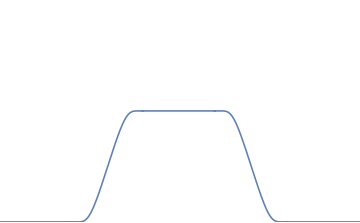
\includegraphics[scale=1]{img/flat.png}};
%\draw (-8,-7.75)-- (8,-7.75);
%\draw[-,dashed] (-5,0)-- (5,0); 
%\draw (-6,0) node[anchor=north] {$1$};
%\draw[-,dashed] (-7,-8.25) -- (-7,-7.25);
%\draw (-7,-8.5) node [anchor=north] {$a$};
%\draw[-,dashed] (0,-8.25) -- (0,-7.25);
%\draw (0,-8.5) node [anchor=north] {$b$};
%\end{tikzpicture}

